% Sample file for 'CACM - Research Highlights'-type articles
% Created by: Gerry Murray, Elec. Pub. Info. Mgr., Pubs. Dept., ACM HQ, NY.
% (murray@hq.acm.org)
%
% This is "research-highlights-sample.tex" (sample file) V1.1 Sept. 2008
% This file should be compiled with V1.1 of "research4cacm.cls" Sept. 2008
%
% If you have already submitted an article to an ACM/SIGS Conference, and have had your
% article published in one of the 'Proceedings', then you have probably used
% the (ACM/SIGS) 'sig-alternate' class and .tex file.
% Any such 'conference-prepared' source .tex file is 'compatible' with the class file
% 'research4cacm' which you will use to prepare your article for inclusion in the magazine 'CACM'.
%
% Here are the steps to take in order to 'morph' your article from being
% a 'conference' article to one more suitable for inclusion in 'Communications of the ACM'.
%
% 1. Change \documentclass{sig-alternate}  to \documentclass{research4cacm}
%
% 2. Comment out the conference information e.g.  %\conferenceinfo{WOODSTOCK}{'97 El Paso, Texas USA}
%
% 3. Make sure the copyright data is correct e.g. \crdata{0001-0782/08/0200}
%
% 4. Make sure the YEAR is correct e.g. \CopyrightYear{2008} with the current default being �2008�.
%
% 5. Comment out the Classification scheme, general terms and keywords.
%
% 6. If you have mentioned authors in the 'Additional Authors' section you should
%    'move them back' into the byline (so that they appear with all the other authors).
%    ALL authors, in Research Highlights articles, get equal billing.
%
% 7. Suitably edit the file (i.e. body text) so as to make it more appropriate for a wider audience.
%
% If, early on in the editorial process, the 'correct' copyright data becomes available
% please change the copyright data to suit, otherwise leave the default '0001-0782/08/0X00'.
% (The editorial staff will change it later on in the production cycle.)
%
% ================= IF YOU HAVE QUESTIONS =======================
% Technical questions _only_ to
% Gerald Murray (murray@hq.acm.org)
% ===============================================================
% ---------------------------------------------------------------------------------------------------------------
%
\documentclass{research4cacm}
\usepackage{epsfig,longtable}
\usepackage{times}
\usepackage{latexsym}
\usepackage{fancybox,subfigure}
\usepackage[normalem]{ulem}
\usepackage{amsmath}
\usepackage{amssymb}
\usepackage{mathrsfs}
\usepackage{verbatim}
\usepackage{appendix}
\usepackage{color}

%\usepackage{natbib}
\usepackage{hyperref}
\usepackage{bnf}
%\bibliographystyle{plain}

\newcommand{\remove}{}
\newcommand{\old}[1]{}
\newcommand{\match}{\stackrel{M}{=}}
\newcommand{\ncite}[1]{$^{\mbox{\tiny \cite{#1}}}$}
%\newcommand{\ncite}[1]{\cite{#1}}
\newcommand{\frags}{{\cal F}}
\newcommand{\snips}{{\cal S}}
\newcommand{\A}{{\tt A}}
\newcommand{\B}{{\tt B}}
\newcommand{\gap}{{\tt -}}
\newcommand{\ideas}{\vskip 0.6cm {\bf IDEAS:\ }}
\newcommand{\motivation}{\vskip 0.6cm {\bf MOTIVATION:\ }}
\newcommand{\mcost}[2]{#1 #2}
\newcommand{\ali}{$\mbox{ }$\hspace{0.2in}}
\newcommand{\acomment}[1]{\hspace{1in}\#{\em #1}}
\newcommand{\beqn}{\begin{equation}}
\newcommand{\eeqn}{\end{equation}}
\newcommand{\captionsize}{\footnotesize}
\newcommand{\LtoN}[1]{\parallel #1 \parallel_{2}}
\newcommand{\mecca}{HapCUT$\:$}
%%%%%%%%%%%%%% FIGURE within a box
\newenvironment{boxfig}[1]{\fbox{\begin{minipage}{\linewidth}
                        \vspace{1em}
                        \makebox[0.025\linewidth]{}
                        \begin{minipage}{0.95\linewidth}
                        #1
\end{minipage}
                        \end{minipage}}}
                                                                                                                                                                            
\def\ensuretext{\textrm}
\newcommand{\Reads}{\ensuretext{{\sc Reads}}}
\newcommand{\AlignStr}{\ensuretext{{\sc AlignStr}}}
\newcommand{\Intervals}{\ensuretext{{\sc Intervals}}}
\newcommand{\Strand}{\ensuretext{{\sc Strand}}}
\newcommand{\Partner}{\ensuretext{{\sc Partner}}}
\newcommand{\MST}{\ensuremath{\mathit{MST}}}
\newcommand{\dist}{\ensuremath{\mathit{dist}}}
\newcommand{\TG}[2]{\ensuremath{\mathit{#1}^{(#2)}}}
\newcommand{\CC}{\ensuremath{\mathcal{CC}}}
\newcommand{\psubs}{\stackrel{\subset}{+}}
\newcommand{\rs}{\ensuremath{\mathit{R_s}}}
\newcommand{\MEC}{\ensuremath{\mathit{MEC}}}
\newcommand{\Prob}{\ensuremath{\mbox{Pr}}}
\newcommand{\fref}[1]{\mbox{Figure~\ref{#1}}}
\newcommand{\secref}[1]{\mbox{Section~\ref{#1}}}
\newcommand{\para}[1]{\vspace{2pt}\noindent\mbox{{\bf #1:} }}
\newcommand{\slimfast}{{\sc SlimGene}}

%%%%%%%%%%%%%%%%%%%%%%%%%%%%%%%%
% GenomeQL syntax
%%%%%%%%%%%%%%%%%%%%%%%%%%%%%%%%%%%
\newcommand{\MapRel}{\ensuremath{\:\overline{\bowtie}\:}}
%\newcommand{\MapRel}{\ensuremath{\stackrel{\bowtie}{\llcorner\lrcorner}}}
\newcommand{\NatJoin}{\ensuremath{{\bowtie}}}
%\newcommand{\MapRel}{\ensuremath{\bowtie_M}}
\newcommand{\Project}[1]{\ensuremath{\Pi_{#1}}}
\newcommand{\ProjectInterval}[1]{\ensuremath{\Pi^i_{#1}}}
\newcommand{\Select}[1]{\ensuremath{{\displaystyle \sigma_{#1}}}}

\newcommand{\gqlSelect}{{\sc select}}
\newcommand{\gqlFrom}{{\sc from}}
\newcommand{\gqlWhere}{{\sc where}}
\newcommand{\gqlAnd}{{\sc and}}
\newcommand{\gqlAvg}{{\sc avg}}
\newcommand{\gqlMin}{{\sc min}}
\newcommand{\gqlMax}{{\sc max}}
\newcommand{\gqlIn}{{\sc in}}
\newcommand{\gqlAbs}{{\sc abs}}
\newcommand{\gqlCount}{{\sc count}}
\newcommand{\gqlGroupby}{{\sc groupby}}
\newcommand{\gqlIntersects}{{\sc intersect}}
\newcommand{\gqlMapjoin}{{\sc mapjoin}}
\newcommand{\gqlProjectInterval}{\gqlSelect\ {\sc merged}}
\usepackage{latexsym}

%%%%%%%%%%%%%%%%%%%%%%%%%%%%%  THEOREM-LIKE ENVIRONMENTS
                                                                                                                                                                            
\newtheorem{THEOREM}{{\bf  Theorem}}
\newenvironment{theorem}{\begin{THEOREM} \hspace{-.85em}  {\bf :} }%
                        {\end{THEOREM}}
\newtheorem{LEMMA}[THEOREM]{Lemma}
\newenvironment{lemma}{\begin{LEMMA} \hspace{-.85em} {\bf :} }%
                      {\end{LEMMA}}
\newtheorem{COROLLARY}[THEOREM]{Corollary}
\newenvironment{corollary}{\begin{COROLLARY} \hspace{-.85em} {\bf :} }%
                          {\end{COROLLARY}}
\newtheorem{PROPOSITION}[THEOREM]{Proposition}
\newenvironment{proposition}{\begin{PROPOSITION} \hspace{-.85em} {\bf :} }%
                            {\end{PROPOSITION}}
\newtheorem{CLAIM}[THEOREM]{Claim}
\newenvironment{claim}{\begin{CLAIM} \hspace{-.85em} {\bf :} }%
                      {\end{CLAIM}}
\newtheorem{OBSERVATION}[THEOREM]{Observation}
\newenvironment{Observation}{\begin{OBSERVATION} \hspace{-.85em} {\bf :} }%
                      {\end{OBSERVATION}}
\newtheorem{DEFINITION}{Definition}
\newenvironment{definition}{\begin{DEFINITION} \hspace{-.85em} {\bf :} }%
                           {\end{DEFINITION}}
\newcommand{\QED}{\hfill$\clubsuit$ \vskip 0.1cm}
%\newenvironment{proof}{\noindent {\bf Proof:} \hspace{.677em}}{\QED}
\newenvironment{packed_enum}{
\begin{enumerate}
  \setlength{\itemsep}{1pt}
  \setlength{\parskip}{0pt}
  \setlength{\parsep}{0pt}
}{\end{enumerate}}
\newenvironment{packed_itemize}{
\begin{itemize}
  \setlength{\itemsep}{1pt}
  \setlength{\parskip}{0pt}
  \setlength{\parsep}{0pt}
}{\end{itemize}}

\begin{document}
%
% --- Author Metadata here ---
% Conference information is NOT appropriate for CACM so comment it out.
%\CopyrightYear{2008} % Allows default copyright year (2008) to be over-ridden - IF NEED BE.
%\crdata{0001-0782/08/0X00}  % Allows default copyright data (0001-0782/08/0X00) to be over-ridden - IF NEED BE.
% --- End of Author Metadata ---

\title{ Abstractions for Genomics: Or, which way to the Genomic Information Age?
% \titlenote{(This is a simple titlenote.)For use with research4cacm.cls. Supported by ACM.}
%
% Show use of \thanks - which can appear here (normal/default) or down by the author
%\thanks{The original version of this paper is entitled ``XXX" and was
%published in (Title of publication, publication date, publisher.)}
%}
%\subtitle{[Extended Abstract]
%\titlenote{A full version of this paper is available in...}
}
%
% You need the command \numberofauthors to handle the 'placement
% and alignment' of the authors beneath the title.
%
% For aesthetic reasons, we recommend 'three authors at a time'
% i.e. three 'name/affiliation blocks' be placed beneath the title.
%
% NOTE: You are NOT restricted in how many 'rows' of
% "name/affiliations" may appear. We just ask that you restrict
% the number of 'columns' to three.
%
% Use the \alignauthor commands to handle the names
% and affiliations.
%
\numberofauthors{6} %  in this sample file, there are a *total*
% of SIX authors and all of them fit neatly on the first page.
% As said, all authors get 'equal billing' and you should fit all of them on the opening page
% in the 'byline'. The production/editorial-staff will 'separate' names from their affiliations, leaving
% author names beneath the title (in the byline), and moving the affilations/contact information to an area
% after the references at the back of the article.
%
\author{
% You can go ahead and credit any number of authors here,
% e.g. one 'row of three' or two rows (consisting of one row of three
% and a second row of one, two or three).
%
% The command \alignauthor (no curly braces needed) should
% precede each author name, affiliation/snail-mail address and
% e-mail address. Additionally, tag each line of
% affiliation/address with \affaddr, and tag the
% e-mail address with \email.
%
% 1st. author
\alignauthor
Vineet Bafna\\
       \affaddr{Computer Science and Engineering, UC San Diego}
       % 2nd. author
\alignauthor
Alin Deutsch\\
       \affaddr{Computer Science and Engineering, UC San Diego}
       % 3rd. author
\alignauthor 
Andrew Heiberg\\       
       \affaddr{Computer Science and Engineering, UC San Diego}
\and  % use '\and' if you need 'another row' of author names
% 4th. author
\alignauthor 
Christos Kozanitis\\
       \affaddr{Computer Science and Engineering, UC San Diego}
       % 5th. author
\alignauthor Lucila Ohno-Machado\\
       \affaddr{Division of Medical Informatics, UC San Diego}
% 6th. author
\alignauthor George Varghese\\
       \affaddr{Computer Science and Engineering, UC San Diego}
}

\maketitle
\begin{abstract}
  With DNA sequencing costs dropping below \$$1,000$ for human
  genomes, the hope is that medicine will be personalized, based on the
  individual's genetic makeup.  As hardware costs fall, software
  costs are a major obstacle to both discovery and personalized
  medicine.  We propose attacking this obstacle using
  a hierarchical set of abstractions (akin to Internet layers)
  for genome processing.  While interface formats exist for mapped
  files (BAM) and variants (VCF), we propose a new separation of
  variant calling into a deterministic evidence layer queried
  by a statistical inference layer via a proposed Genome Query
  Language (GQL).  GQL allows inference engines to efficiently sift only the
  relevant evidence (e.g., the READs that flank a SNP site) from raw
  genomic data. Using a set of exemplar queries, we argue that the
  standard implementation of GQL using relational database tables with
  billions of rows for each genomic location will not scale; instead,
  we introduce efficient indices based on compressed strength vectors.
  We outline several benefits to separating evidence from inference
  including the ability to reuse genomic data, and enabling a shift from deep
  analysis of individual genomes to group inference on large
  populations.  Our paper is written for computer scientists: it
  starts with an introduction to genomics and ends with a set of challenges in computer systems,
  security, information retrieval, inference, and databases.
\end{abstract}


\section{Universal Sequencing}

We are a product of ``nature and nurture''. By this, we mean that our
\emph{phenotype} (the composite of all outward, measurable,
characteristics including our health parameters) is a function of two
things: our \emph{genotype} (the DNA program inside all cells), and
the environment (all inputs to a human such as food and
medicine).  This is analogous to
how the output of a program (e.g., a search engine) is
a function of both the program and the input (keywords typed by
user). Using the same input with a different program
(e.g. Google search vs. Bing) can result in different
output.

In this analogy, the role of the medical professional is to provide
information that is either ``diagnostic'' (i.e. is there a bug in the
program based on observed output?), ``prognostic'' (e.g., can we
predict the output/outcome, given specific inputs such as diet?), or
``therapeutic'' (e.g., can any specific input such as a drug lead to
the desired output). Also, the Electronic Medical Record (EMR) of a
patient can be described as an archive of previously acquired inputs
and outputs.  

\old{While this is a useful analogy, there are subtle
differences.  Unlike computers, the human hardware (the body) itself
is the output of programmed instructions and previously received
input; thus, each program runs on unique and constantly changing
hardware.  Additionally, the program itself changes over the course of
the lifetime of the individual due to acquired mutations in the DNA,
but we will not discuss this here.}

Unlike computers, the human ``program'' was largely hidden away. As a consequence, medicine has
traditionally been ``depersonalized'' with doctors providing
treatments by comparing the patient's phenotype (symptoms)
against empirical observations of outputs from a large number of
individuals.  There was only limited customization based on
on coarse classes such as `race'.  All of this changed with the sequencing of
the human genome in early 2000, and the subsequent drop in costs from
hundreds of millions of dollars down to \$1000 on small desktop
sequencing machines. The ability to cheaply read the program of each
human underlies the great promise of \emph{personalized medicine}---
treatments based on symptoms and the patient's distinctive DNA program.

We frame this point with a classic example. The blood-thinner drug,
Warfarin, is widely prescribed to prevent blood clots. The dosage is 
critical: too high, and the
patient can bleed to death; too low and the drug may not prevent
life-threatening blood-clots. Often, the right dosage is established
through multiple visits to the clinic and regular testing. However,
recent reports~\cite{Schwarz2008} suggest that knowledge of the
patient's genetic program can help establish the right dosage. This
approach (Genetic association or a \emph{discovery workflow}) is
outlined below.
\begin{packed_itemize}
  \item Collect a sample of affected, and `genetically matched' control individuals; sample DNA, and catalog variations.
  \item Identify and  report variations that co-segregate (i.e., correlate) with the affected/control status of the individual.
  \item Follow up on the genetic basis of the correlation through
    expensive follow-up studies and experiments in animal models
    and clinical trials. Transfer knowledge to the clinic.
\end{packed_itemize}
Even with its successes, the discovery approach has problems.
First, studies are resource-intensive and require
identifying and sequencing large cohorts of
individuals with and without a disease. Second, it is unclear how to
apply the study results to a specific individual, especially one that
is genetically different from the investigated cohort.  Finally, data
reuse is difficult: significant computation must be
expended to dig out data from a previous study and much care
is required to reuse the data. We contrast the discovery
work flow with \emph{personalized medicine}. Here, a physician
treating individual $A$ may query a database either for: treatments
suitable for patients who have genetic variations similar to those of
$A$; or query for patients genetically similar to $A$ for treatments
and dosages that worked well for these patients.

The notion of computational tools enabling personalized
medicine is gaining currency.  Some groups have proposed specialized
databases for cancer genomes (e.g., \cite{Patterson2011}) although
specific details are still emerging.
Here, we take a more general viewpoint, arguably allowing for
broader access to genomic information, and enabling both discovery and
personalized medicine.

\textcolor{blue}{Specifically, we start with a shift in perspective
  that is implicit in the personalized genomics community. Instead of
  sequencing small cohorts on a need-to basis, this new vision assumes
  that each individual is sequenced at birth, and her personal genome
  is an integral part of her EMR (medical record), and available to be
  queried by trained researchers and medical personnel. This scenario
  is realistic considering the rapid drop in sequencing costs.}


In the example of choosing Warfarin dosage for a patient, the medical
team might do the following: (a) identify a collection of individuals
genetically similar to the patient and on a warfarin regimen; (b)
query their genomes and EMRs for genetic variation in candidate genes
and warfarin dosage, respectively; and, (c) choose the appropriate
dosage based on the patient's specific genetic program. The ability to
logically select from a very large database of individuals using the
phenotype as a key removes the first problem described with the
discovery workflow.  Using genetic variations specific to an
individual $A$ as a key to return treatments (that work well for such
variations) addresses the second problem.  Finally, if the
accompanying software system has good abstractions, then the third problem 
(computational burden to reuse
data) is also greatly eased. 

\textcolor{blue}{We start with the assumption that the genome sequence
  of all individuals is available to be queried, and claim (along with
  other personalized medicine researchers) that this shift in
  perspective (see Figure~\ref{fig:fig1}) enables personalized
  medicine and large-scale discovery}. Our paper focuses on proposing key software
  abstractions for genomics-- we suggest that like other CS areas
  (VLSI/Systems), software abstractions will enable genomic medicine.
  \old{along with efficient implementations.  In computer science, key
    abstractions such as virtual memory and relational data models
    have vastly improved productivity and reduced software costs to
    keep pace with cheap VLSI hardware: our central thesis is that the
    same is required for genomics.}



\begin{figure}[htbp]
  \centering
  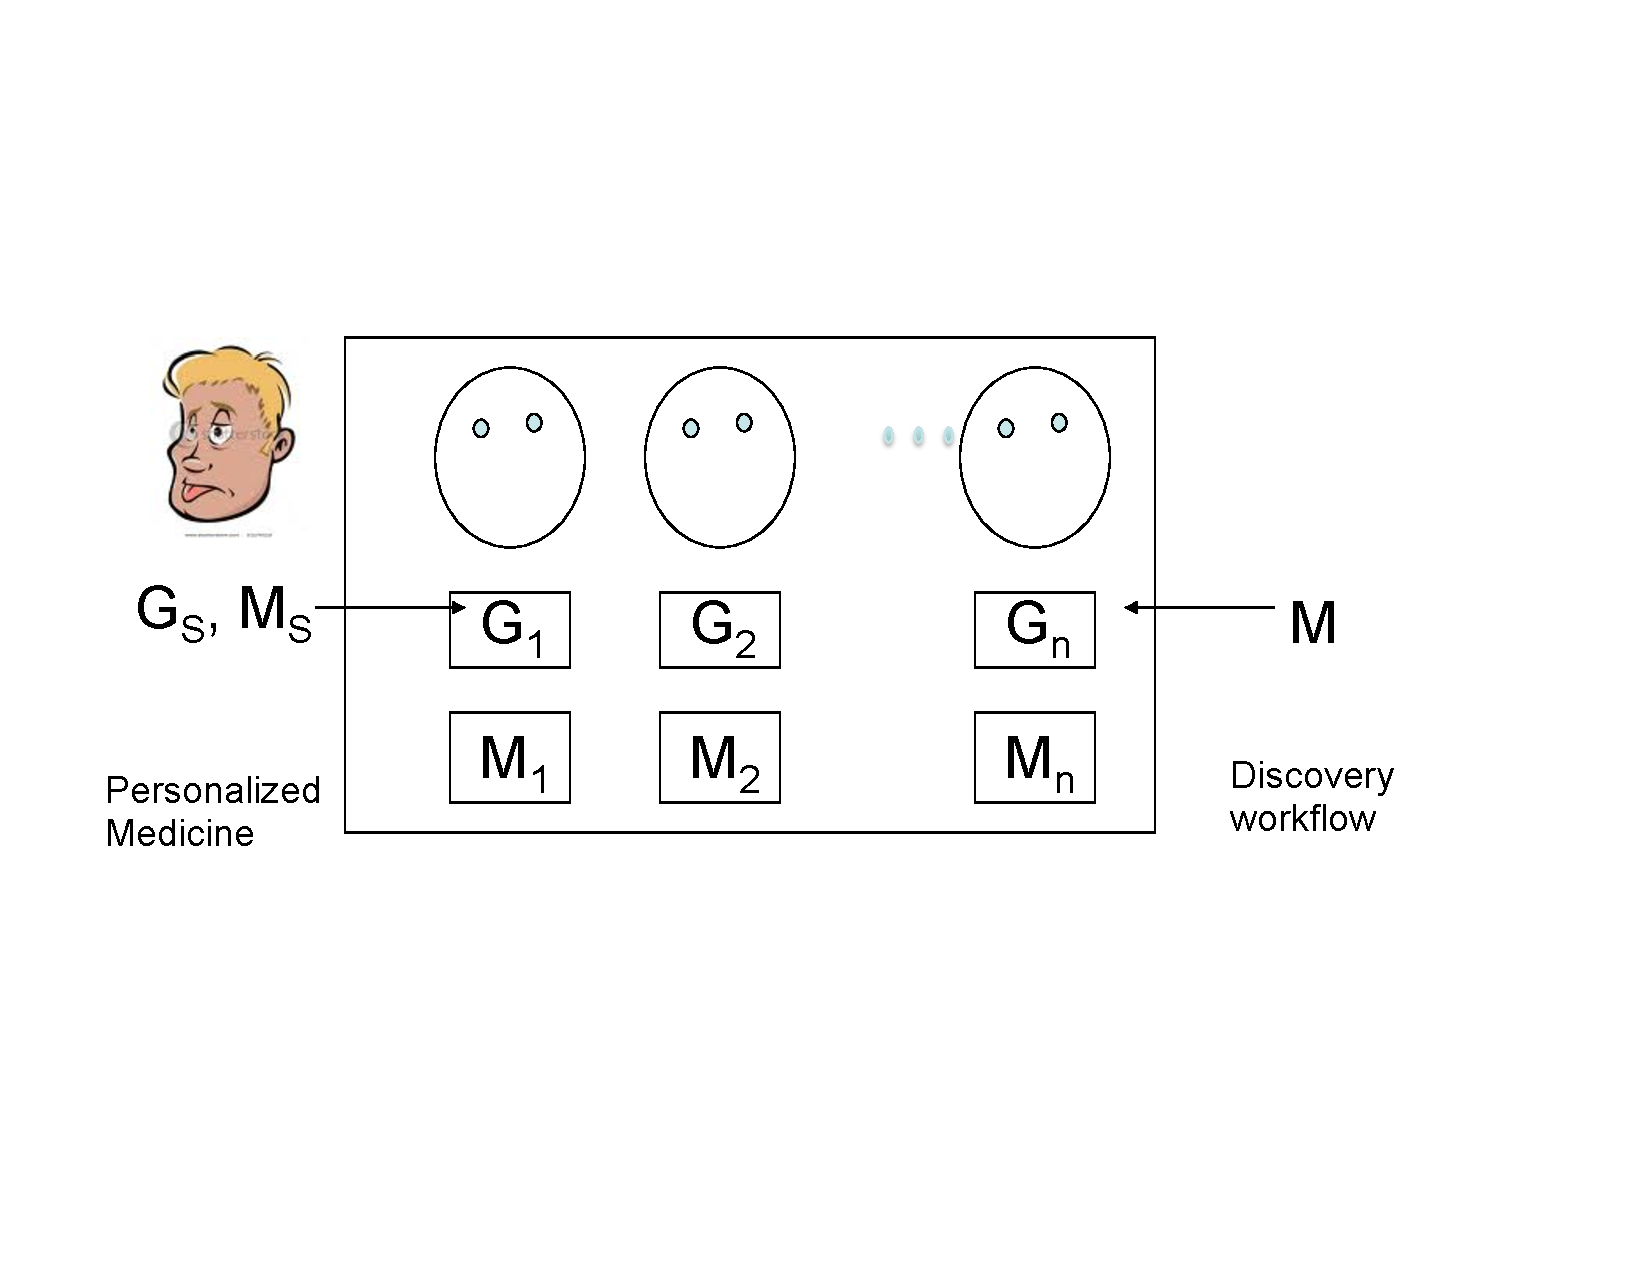
\includegraphics[trim = 15mm 70mm 20mm 50mm, clip, width=3in]{fig/personalizedmedicine.pdf}
  \caption{{\bf Universal Sequencing, discovery, and personalized medicine}. Assume 
    every individual is sequenced at
    birth. In discovery, we logically select a
    subset of individuals with a specific phenotype (e.g., disease)
    and another without the phenotype, and then identify genetic
    determinants for the phenotype. By contrast, in personalized medicine
    we retrieve the medical records of all patients genetically similar to a sick patient
    S.}
  \label{fig:fig1}
\end{figure}
\old{
Further, computer systems designers often benefit from systems
thinking: making tradeoffs at the component level for overall
benefits, and leveraging technology trends. We will argue that system
thinking is badly required in genomics because genomic processing was
invented in an era of scarcity, where genomes were scarce and
sequencing was expensive; the time has come to rethink these
assumptions.  This article is written so that computer scientists ---
not just bioinformaticians who have already contributed so much, but
computer scientists of every ilk and especially computer systems
researchers --- can engage with biologists and doctors in an essential
endeavor to improve the health of the planet.


We note upfront that new genomic technologies are also helpful in
sampling the dynamic states of the cell. For example, transcript
sequencing technologies (e.g. RNAseq) provide a direct look at which
genes might be activated, or repressed in specific contexts. Likewise,
other technologies probe the cell from a systems biology viewpoint
decoding networks of interacting proteins, RNA, and DNA (See
Section~\ref{sec:genetics}) for definitions. }

We start by describing basic genetics using programming metaphors in
Section~\ref{sec:genetics}. Section~\ref{sec:trends} describes trends
in sequencing.  We describe how genetic variations are called today in
Section~\ref{sec:usecases}.  Our vision for a vast genomic database
built in layers is described in Section~\ref{sec:vision}--- the key
idea is the separation of `evidence' and `inference'.  In
Section~\ref{sec:gqa}, we propose a language for specifying genome
queries.  We end in Section~\ref{sec:futuredirections}) by outlining
research directions for other areas of computer science to further
this agenda.

{\bf Scope:} We limit our scope to genomics, ignoring dynamic aspects
like transcript, protein expression, and pathway databases.  Genomic
information is traditionally analyzed using two complementary
paradigms. First, {\em comparative genomics}, where different species
are compared-- most regions are dissimilar, and the conserved regions
are functionally interesting~\cite{Haussler2009, Haussler2011}. The
second approach is {\em population genomics}, where genomes from a
single population are compared under the baseline hypothesis that the
genomes are identical and it is the variations that define phenotypes
and are functionally interesting.  Our paper focuses on population
genomics and its application to personalized medicine. Finally, we do
not discuss specific sequencing technologies such as strobe sequencing
versus color space encoding.
                    


\section{Genetics for Computer Scientists}
\label{sec:genetics}
We provide a quick introduction to genetics for computer scientists; 
a standard reference such as ~\cite{Alberts2007} can provide more
details.

All living creatures consist of cells; each cell is like
a computer running a program which is its DNA. The program uses 3
billion characters (\emph{nucleotides/basepairs}) from a fixed
alphabet $\{A,C,G,T\}$. Humans are {\em diploid} --- there are two
programs controlling each cell, one inherited from the father and one
from the mother.  Further, each program is broken up into $23$
``modules'' called chromosomes and within each chromosome are sparsely
scattered small functional blocks called genes. The module pairs from
the father and mother are called homologous chromosomes and each human
has a pair of (homologous) genes from each parent.


The `hardware' of the cell consists of cellular organelles
and proteins--- the cellular machinery. Proteins perform specific
cellular functions such as catalyzing metabolic reactions and transducing
signals. The gene contains the `code' for manufacturing
proteins. Each gene executes in one of many `ribosomes' (analogous to
a CPU).  Information travels from the nucleus (where the packaged DNA
resides) to the ribosome via a `messenger' molecule (mRNA) that is
essentially a copy of the coding DNA. The ribosome `reads' the code 3
bases (one codon) at a time. Each codon is analogous to an OpCode
instructing the ribosome to attach a specific amino acid to the
protein sequence being constructed. Thus, the DNA program provides
instructions for making the hardware which in turn performs all
cellular functions.

A change (\emph{mutation}) in the DNA can change the amino-acid, and
correspondingly, the cellular machinery resulting in a different
phenotype (output). In the Mendelian paradigm, each of the two
homologous copies of the gene controls one {\em phenotypic trait}
(e.g., ability to clot blood). A mutation in one gene might impact the
phenotype strongly (\emph{dominant}), not at all (\emph{recessive
  mutation}) or somewhere in between. In fact, most phenotypes are
\emph{complex}--controlled by the paired copies of multiple
genes. Nevertheless, DNA controls traits so even the simplest queries
on DNA are useful --- e.g., {\em Compared to a `normal' individual,
  are there parts of the patient's DNA program that have mutated}.

Advancements in sequencing has made it possible to cheaply scan an
individuals genetic program for mutations (or, \emph{variations}).
First, a physical process is used to randomly shear genomic DNA into
small \emph{inserts} of size $500$-$10000$bp. The sequencing machine
deciphers the DNA from small \emph{fragments, or reads} (length
$L\simeq 100$bp) at one or both ends of the inserts.  Thus, the
genomic information is presented as a collection of small strings over
A,C,G,T, sampled from a random location on a (maternal or paternal)
chromosome. It is natural to assume that these fragments will be
assembled like a giant jigsaw puzzle.  However, this is complex and
expensive because of the large amounts of repetitive portions in human
genomes.

{\bf Mapping, and Variation:} An alternative to assembly used today is to
\emph{align}, or \emph{map} the non-repetitive fragments of a sampled
genome (the \emph{donor/patient genome}) to a reference human genome.  The
current reference is a single (haploid) copy of each chromosome
sampled from multiple individuals. Mapping involves finding a location
on the reference where the genomic substring matches the query
fragment up to a small number of errors. The errors might be
sequencing errors or true variations in the query, relative to the
reference. Mapping works because string search is more tractable than
assembly and any pair of human genomes is identical to 1 in $1000$
locations.

A true deviation in the donor sequence relative to the
reference is called a {\em variation}.  The simplest variation is a
\emph{SNV} (single nucleotide or single character variation). Recall that donor genome consists
of two copies.  A variation
that occurs in both copies is called
\emph{homozygous}; a variation that occurs in
only one copy is called {\em heterozygous}. The specific value
of the variant is called an \emph{allele}. For example, suppose that
the DNA at homologous chromosomes of individual $A$ compared to the
reference is as follows
\[
\begin{array}{cl}
\cdots ATG\cdots GAGTA\cdots & \mbox {Reference Assembly}\\
\cdots ACG\cdots GAGTA\cdots & \mbox {Maternal chromosome 1}\\
\cdots ATG\cdots GAGCA\cdots & \mbox{ Paternal chromosome} 
\end{array}
\]
Then, individual $A$ is bi-allelic, or heterozygous at the 2 SNV
sites, has the \emph{genotype} $\cdots C/T\cdots C/T\cdots$, and the
genotypes are resolved into two \emph{haplotypes} $\cdots C\cdots
T\cdots,\cdots T\cdots C\cdots$.

Sites containing SNVs that are prevalent in a population demarcate
chromosomal positions as varying, or polymorphic. Consequently, these
locations are called \emph{SNPs} (Single Nucleotide Polymorphisms). In
discovery workflows, we test populations to see if the occurrence of
variation correlates or \emph{associates} with the phenotype status of
the individual.

So far we have talked of simple variations involving one, or a small
number of changes at a location. By contrast, we also have
\emph{structural variations} in which large (one kbp to several
million bases) genomic fragments are deleted, inserted, translocated,
duplicated, or inverted, relative to the
reference~\cite{Tuzun05}.

\section{Sequencing Trends}
\label{sec:trends}
The following trends are relevant to designing a genomic software architecture:

\begin{itemize}
\item {\em Reducing costs:} While the Human genome project 
  cost $\sim \$100M$, human
  re-sequencing costs for a redundant ($15\times$) coverage are now
  under \$5K, and projected to go below \$1K. This implies
  that universal sequencing may be realizable, and 
  archival and analysis, not sequencing, will dominate
  cost.

\item {\em Small Read lengths:} New sequencing technologies have
  largely sacrificed length and sequence quality to massive
  parallelism and high throughput. \textcolor{blue}{As
    `single-molecule' sequencing technologies come on board, it is
    possible that reads will become long enough ($\sim$ 100Kbp) to
    allow for de novo assembly. Nevertheless, raw reads will continue
    to remain first class entities.}

\item {\em Prohibitive Assembly Costs, Paired end sequencing:} Repetitive regions cover $\sim 40\%$ of the human
  genome. If the read-length is shorter than the length of repetitive
  sequence, the genome cannot be assembled uniquely. Longer reads or
  reads sequenced from ends of long clones (paired end reads) are
  necessary to resolve repeats and assemble sequences \emph {de
  novo}.  Thus, today sequenced reads are mapped to a standard
  human reference to identify variations, and these variations are correlated
to phenotype variation. 

\item {\em Computer System Costs will soon dominate:} Some studies
\cite{Stein2010, Pennisi2011}
  have shown that the costs of disk storage for genomes is now greater
  (and decreasing slower) than the costs of sequencing.  
\end{itemize}

\old{
Therefore, we start with the premise that the genome sequence of an
individual will continue to be in the form of fragments (possibly with
an assembly) in the near future. We start by presenting some
biologically inspired queries. }

We start with some exemplar queries on genomic data that illustrate the difficulty of
genomic analysis and show that there is no
consensus on the best method.  Abstractions must be flexible to handle
a variety of methods.

\section{Variation Calling}
\label{sec:usecases}
The key to efficiency in genomics is the premise that an individual's
genetic record can be summarized succinctly by a much smaller list of
individual genetic variations.  While we develop this premise further
in our layering proposal (Figure~\ref{fig:abstraction}a)), we provide
the reader with intuition as to how variants are
called {\em today}.  The expert should skip this section and proceed
to our layering proposal. We start with querying for Single Nucleotide
Variations (SNVs) in the donor genome, the simplest form of variation.

\subsection{Calling SNVs}
Figure~\ref{fig:variationevidence} shows how a mutation may be called.
Consider the reference allele {\em C}. We see two copies of the donor
genome with a {\em G} allele, and some copies with a {\em C}, indicating
a heterozygous SNV. If the variation is homozygous, we expect all
overlapping READs to have a {\em G} in that position. Even this simple
call can be confounded. First, some of the reads may have been mapped
to the wrong place on the reference; such as the top donor read in the
figure. The G/T mutation may not be correct and the alignment of the
incorrectly mapped read might present many variations. Even if the
READ is mapped correctly, sequencing errors could incorrectly appear as
heterozygous mutations.

Thus, mutation callers use various statistical methods informed by
mapping quality (e.g., the number of potential places in the genome a
read can map to) of the read, the quality score of a base call, and
the distribution of bases or alleles in the READs for that location.
Some mutation callers even use evidence based on the surrounding
locations (e.g., an excess of insertion/deletion events
nearby suggests alignment problems). The decision itself could be
based on frequentist, Bayesian inference, or other machine learning
techniques.  While SNP callers use various inference techniques, they
all use the same evidence: the set of reads overlapping the location
of the SNP in question.
 
\subsection{Calling Structural Variations}
In addition to small nucleotide changes, larger structural variations
involving insertion, deletion, and translocation of large genomic
regions also form an important source of genomic variation. Consider
the example of deletions in the donor genome
(Figure~\ref{fig:variationevidence}b) in which a large segment of DNA
is deleted, relative to the reference). If both copies of the donor
genome are deleted, the deletion is {\em homozygous}; otherwise, it is
{\em heterozygous} deletion. Deletions can be detected using a number
of techniques:

\begin{figure}[htbp]
  \centering
  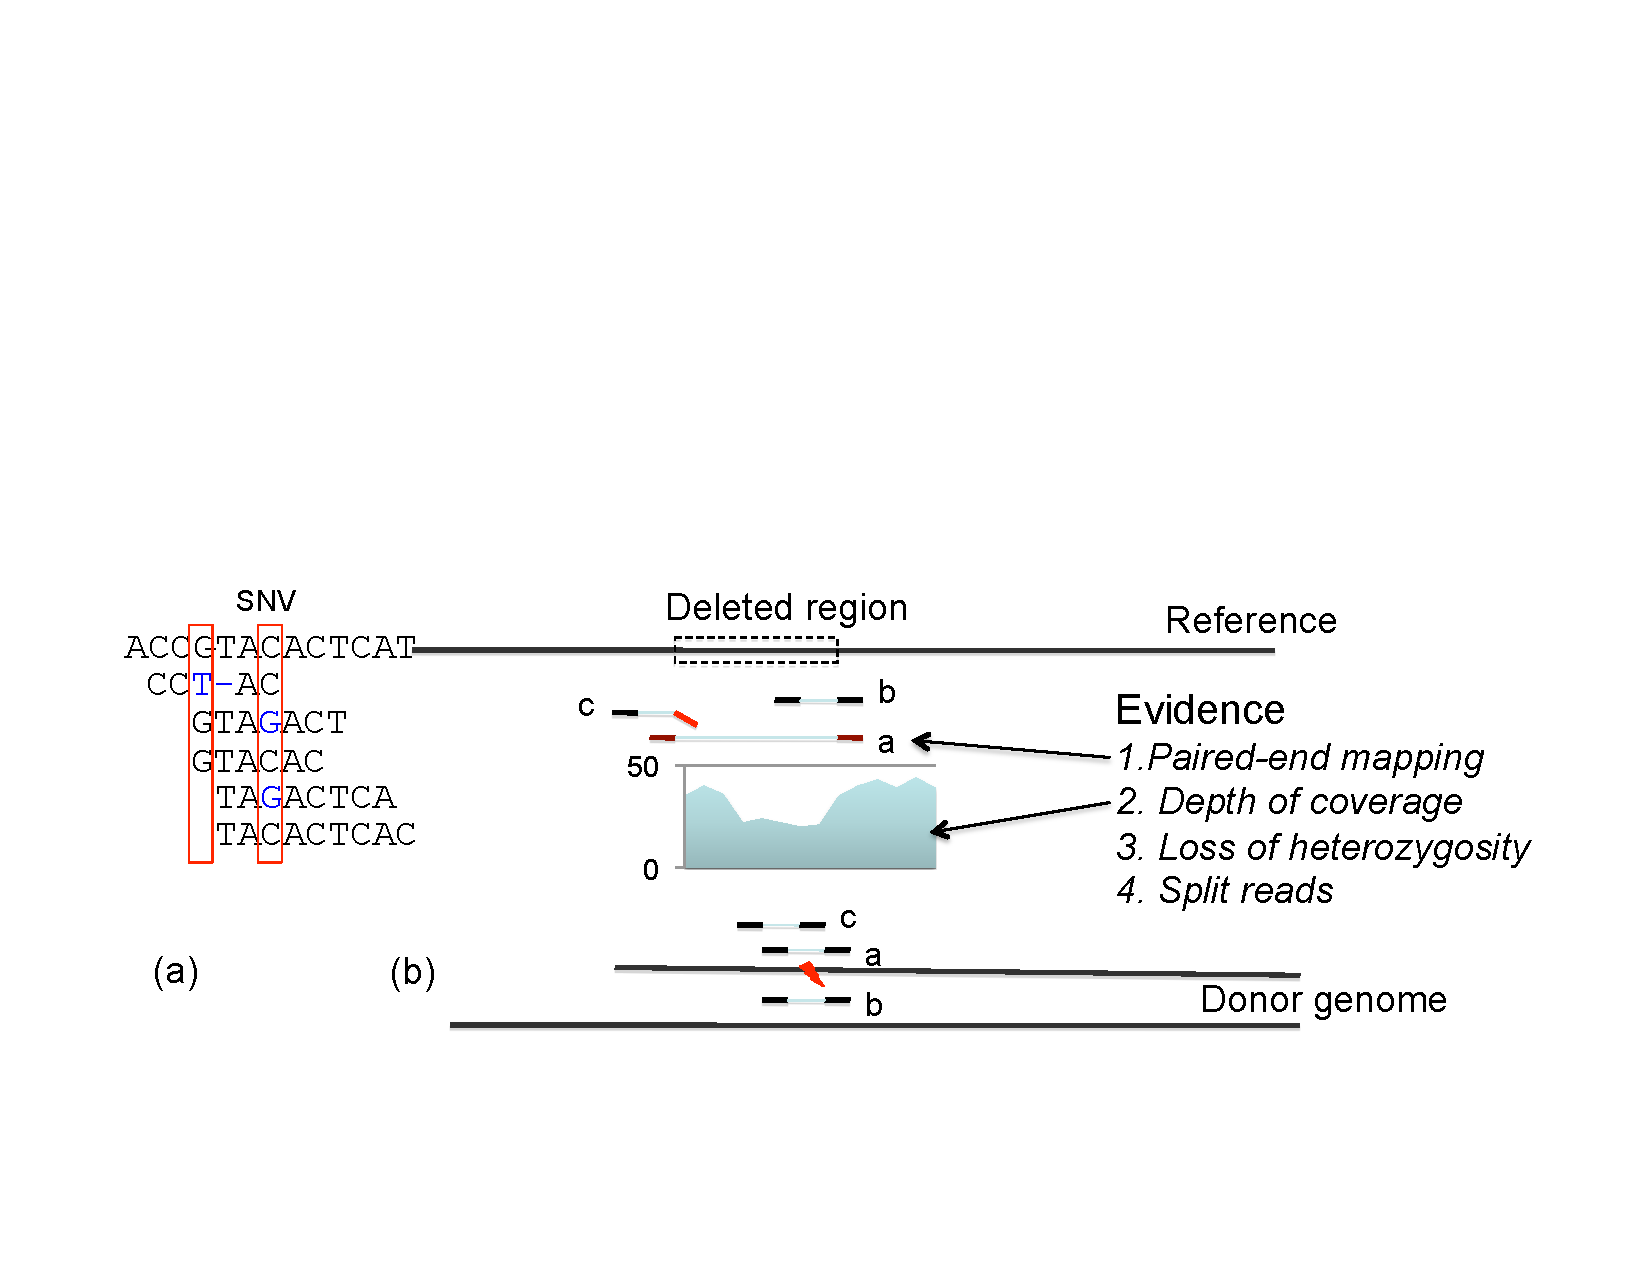
\includegraphics[trim = 5mm 30mm 5mm 100mm, clip, width=3.2in]{fig/deletion_and_SNV_evidence.pdf}
  \caption{{\bf Evidence for variation in the donor}. (a) The evidence
    for SNVs is provided by aligning donor reads against the reference
    sequence. The G/T variation might be a sequencing error as the
    variant reads maps with too many errors. However, the G/C
    variation appears to be a true SNV. (b) Paired-end sequencing and
    mapping provides evidence for deletion in the genome. The dotted
    rectangle demarcates the region in the reference deleted in
    exactly one of the two donor chromosomes. Read `a' samples the
    region around the deletion (marked with the lightning bolt), and
    maps `discordantly' in the reference; read `b' maps concordantly,
    but with coverage about half of neighboring regions; read 'c' is
    sampled from the breakpoint and can map only at one end. }
  \label{fig:variationevidence}
\end{figure} {\bf Paired-end mapping:} In Paired-end sequencing, both
ends of large genomic fragments (sampled randomly from the donor
genome) are sequenced. These genomic fragments have been size-selected
to be tightly distributed around a specified length $L (\simeq
500)$. If paired reads end up mapping much further apart than $L$
(\emph{length-discordance}), we can infer a deletion in the donor
relative to the reference (e.g., read `a' in
Figure~\ref{fig:variationevidence}b). If the deletion is heterozygous,
we should see a mix of concordant and discordant reads at the
breakpoints of the deletion.

{\bf Depth of coverage:} ``Depth'' at a position refers to the count
of reads mapped to the position. Deleted regions of the donor
chromosome will have reduced coverage --- roughly half for
heterozygous deletions and zero for homozygous ones. Thus, read `b' in
Figure~\ref{fig:variationevidence}b maps within the deleted region,
but reads a,c do not.


{\bf Single end mapped, and split-reads:} When a read maps to the
breakpoint of the deletion on the donor, it cannot be mapped back to
the reference (Figure~\ref{fig:variationevidence}b, read `c'). In the
case of a `clean' deletion, the prefix and suffix of the fragment
could be mapped separately, and such split-reads are indicative of
deletion events.

{\bf Loss of heterozygosity:} Consider the SNV locations on the donor
genome. While sampling multiple polymorphic sites, we expect a mix of
heterozygous and homozygous sites. At
a deletion, the single chromosome being sampled displays a loss of
heterozygosity.

Even within these four categories, a number of design decisions are
made by individual tools to account for repetitive sequences, and
reconcile conflicting evidence. Variant inference remains a
challenging research problem.


\old{ Often, the
  occurrence of breakpoints in repeat regions, and the presence of
  non-templated insertions makes this harder, but split reads are
  still useful clues for small deletion events.  } 

\old{
IMPORTANT but poorly placed; also likely to be misinterpreted.
We also note that genomics today is dominated by what we call {\em
  scarcity thinking}.  Three examples of scarcity thinking follow.
First, a human genome is stored using 250 Gbytes of storage which
contrasts poorly with the roughly 6 Gbits required to encode 3 billion
nucleotides.  Even with the best compression, we find that storage is
dominated by a 8-bit quality score per nucleotide.  While this makes
sense in a world of 1 or 2 genomes where every sequenced nucleotide is
precious, it makes no sense in a world of cheap genomes.  Second, a
number of variant callers specialize their calls based on the type of
instrument used to collect the sequence.  While this makes sense in a
world of a few genomes, the resulting loss of modularity has large
software costs.  Third, the relative lack of evidence (coverage of 10
is rare) for any variation, complicates inference today.  However, in
the future thousands of genomes may attest to a correlation between
disease and variation, enabling new inference methods.
}

\section{Layering for genomics}
\label{sec:vision}
Our vision is inspired by analogy with systems and networks.  For example, the
Internet has successfully dealt with a wide variety of new link
technologies (from fiber to wireless) and applications (from email to
social networks) via the ``hourglass'' model using the key
abstractions of TCP and IP (Figure~\ref{fig:abstraction}a). 

Similarly, we propose that Genomic Processing software be layered into
an instrument layer, a compression layer, an evidence layer, an
inference layer, and a variation layer that can insulate genomic
applications from sequencing technology. Such modularity requires us
to forgo efficiencies that can be gained by leaking information across
layers.  For example, biological inferences can be sharpened by
considering which sequencing technology is being used (e.g., Illumina
versus Life Technologies) but we suggest that modularity is paramount.

Some initial interfaces are in vogue.  Many instruments now produce sequence data as
`fastq' format. The output of mapping reads is often represented as
SAM/BAM format, although other compressed formats are being
proposed~\cite{Kozanitis2011}.  At a higher level, 
standards such as VCF are used to describe variants (See Figure~\ref{fig:abstraction}a).

We propose additional layering between the mapped tools and
applications. Specifically, we separate the collection of
\emph{evidence} required to support a query (deterministic, large data
movement, standardized) from the \emph{inference} (probabilistic,
comparatively smaller data movement, little agreement on techniques).
We assert that while Inference methods vary considerably, the Evidence
for inferences is fairly standard. To gather this evidence in a
flexible and efficient manner, we propose a Genome Query Language
(GQL).

While we do not address it, a careful specification of a variation
layer (Figure~\ref{fig:abstraction}a)) is also important.  While the
data format of a variation is standardized using, for example, VCF,
the interface functions are not. 

\old{An application like
personalized medicine or discovery will query the variation layer and
join the variation information with phenotype information gleaned from
medical records (EMRs).}

\begin{figure}[h!]
  \centering
 (a) 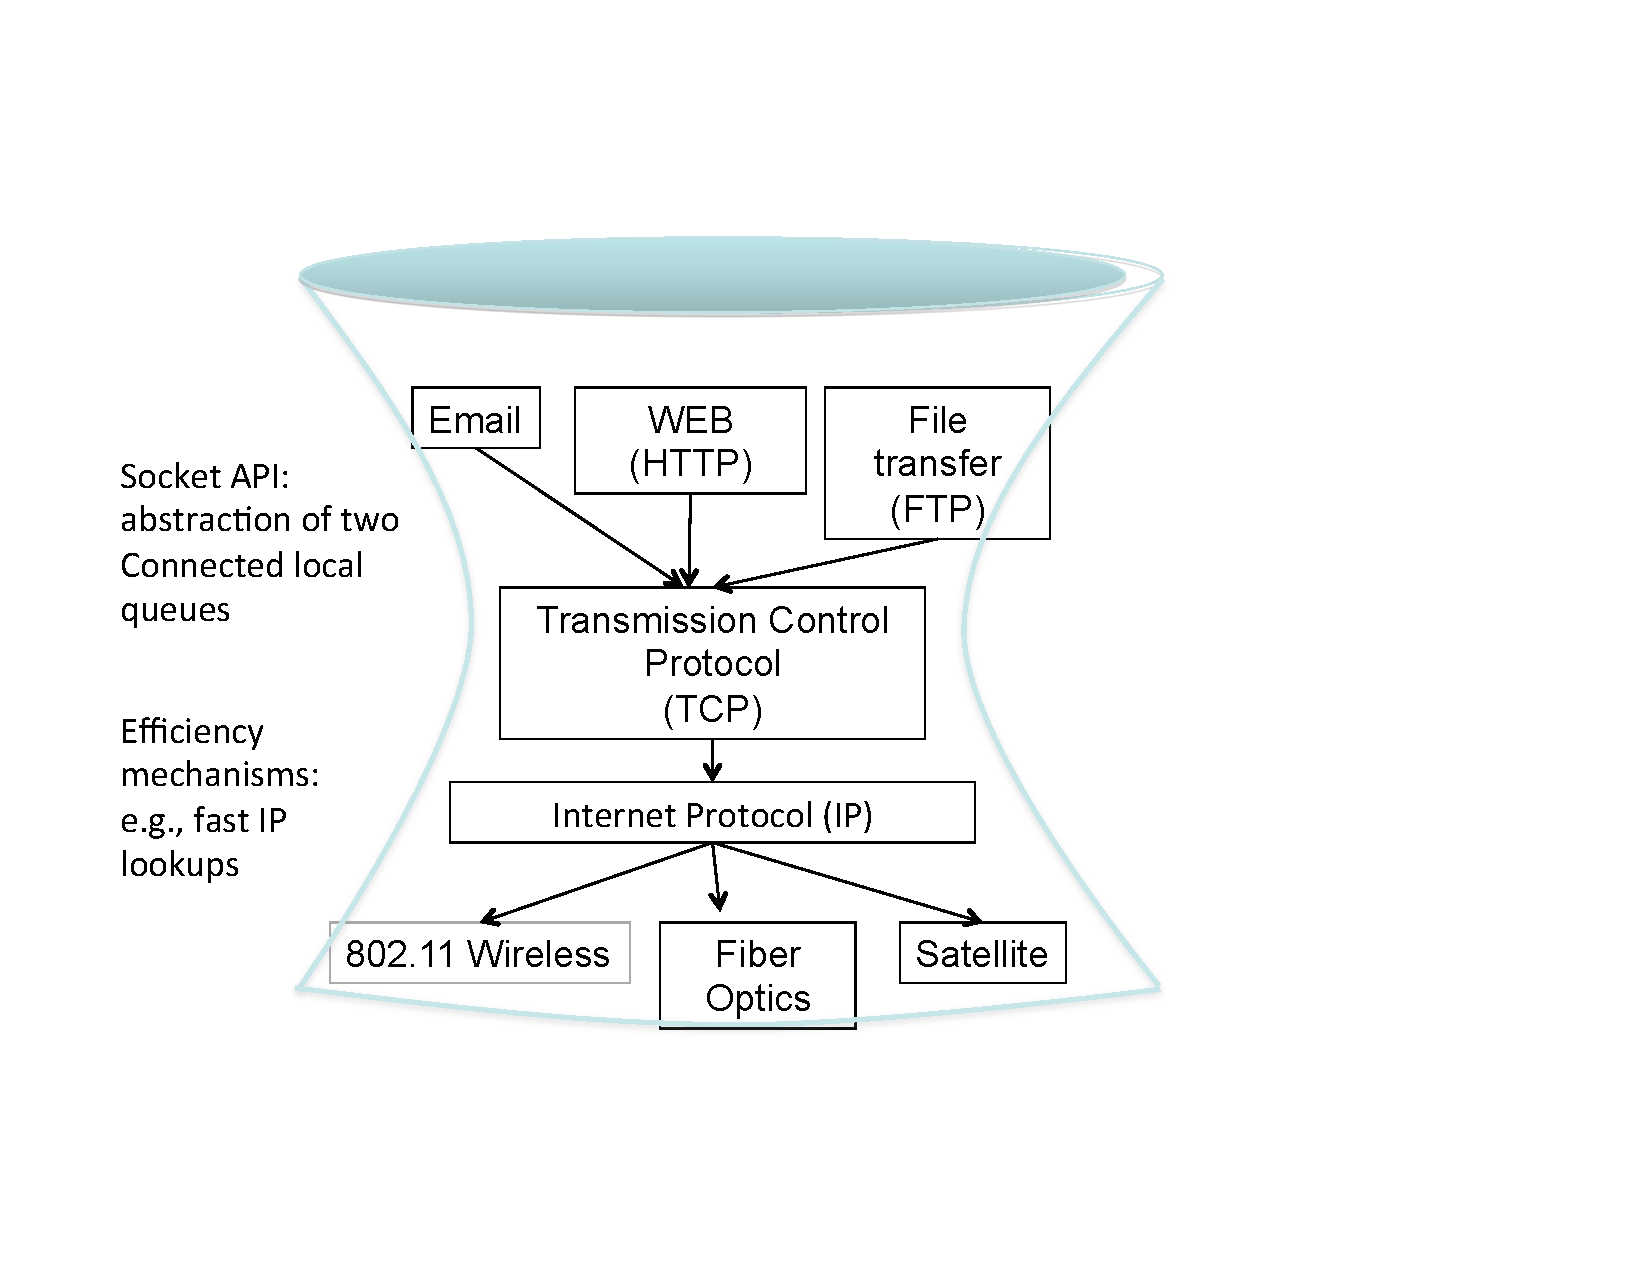
\includegraphics[trim = 0mm 40mm 60mm 10mm, clip, width=1.6in]{fig/hourglass.pdf}
  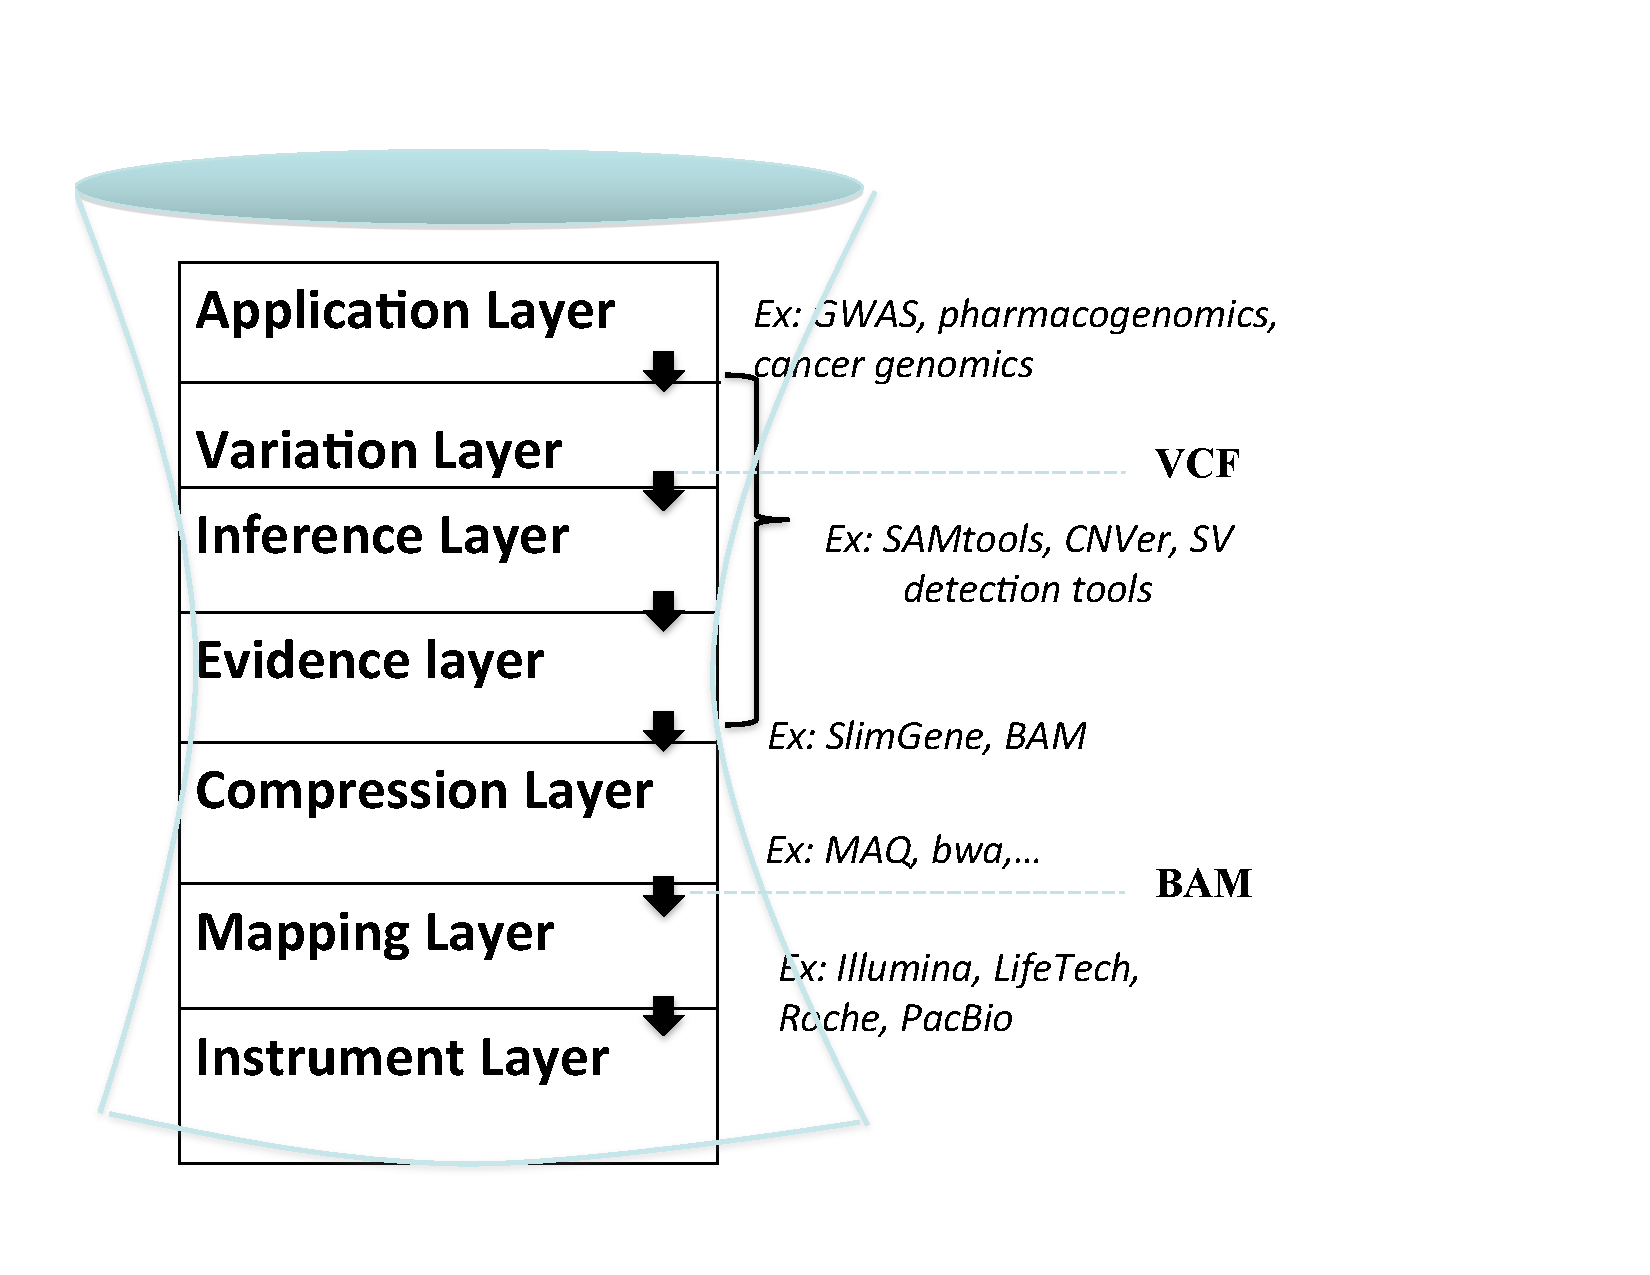
\includegraphics[trim = 0mm 15mm 40mm 10mm, clip, width=1.5in]{fig/genomicabstraction.pdf}\\
 (b) 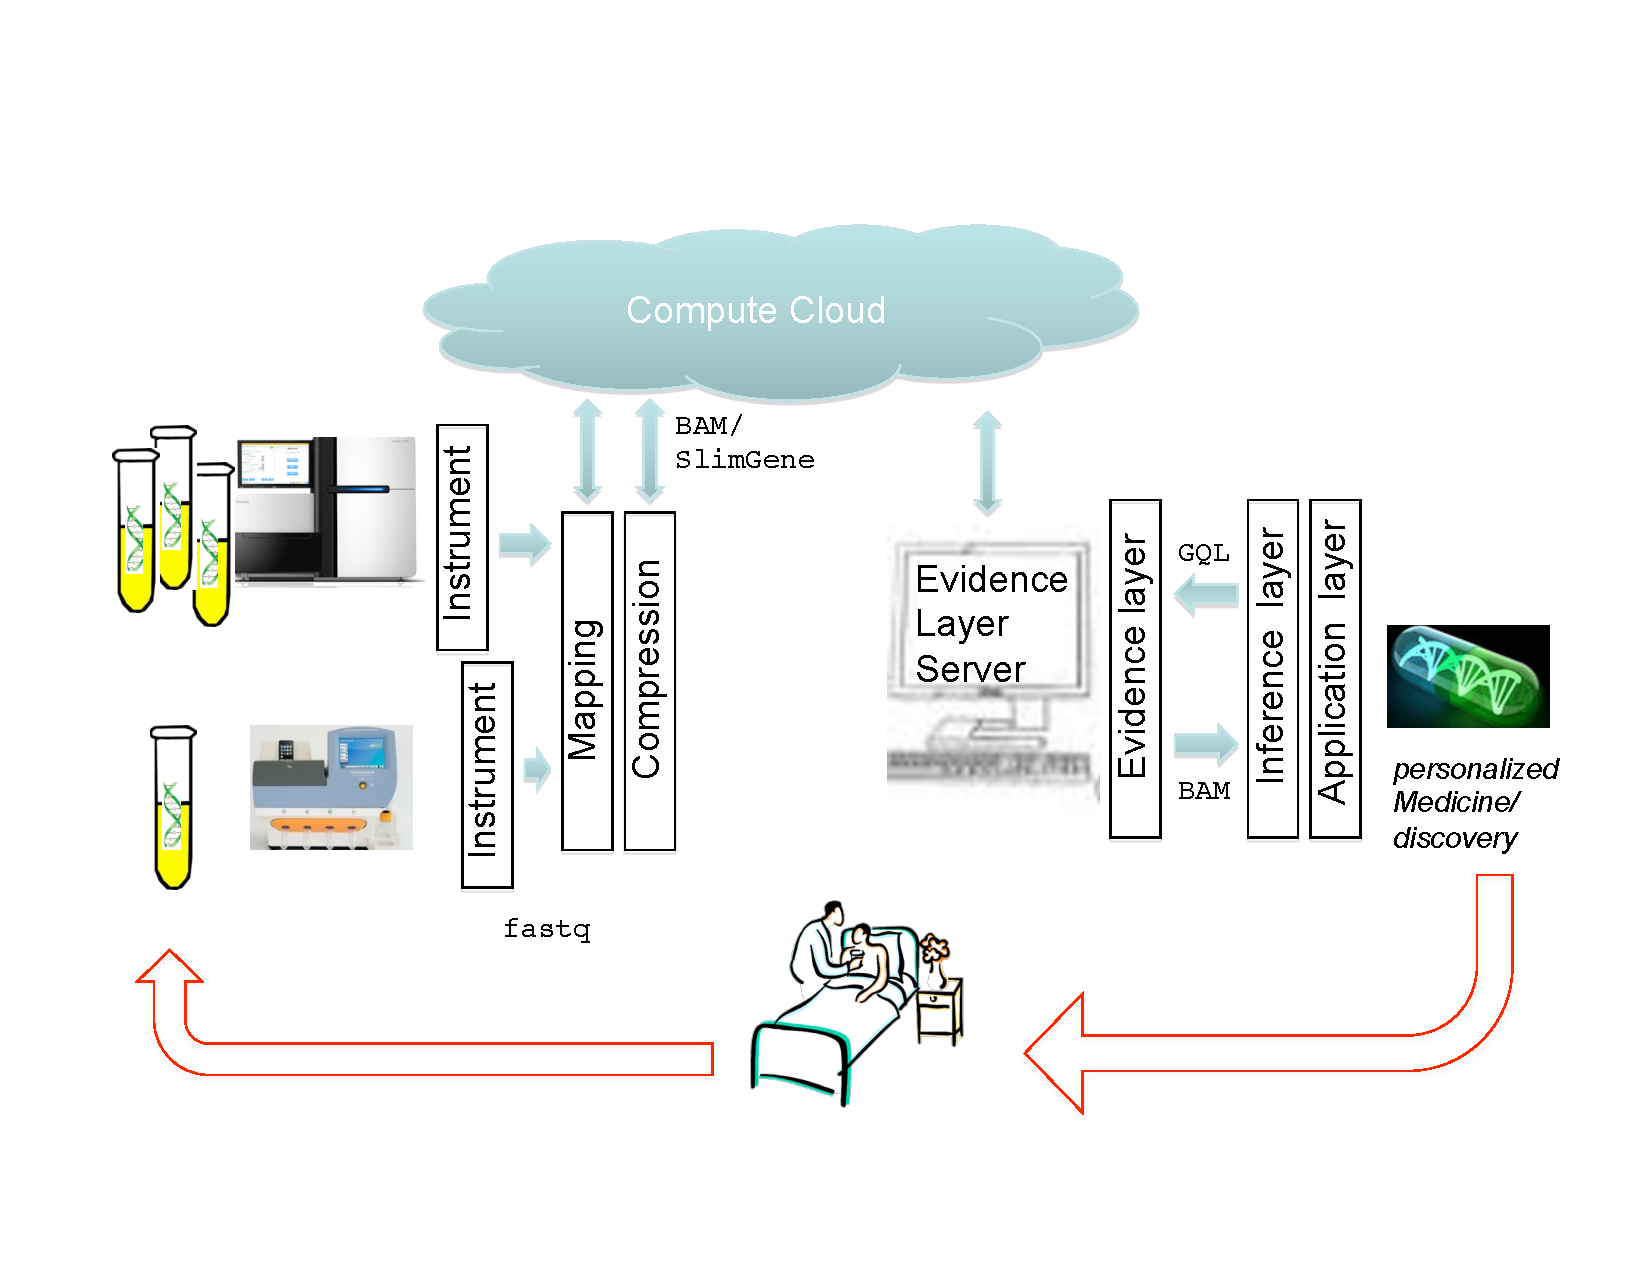
\includegraphics[trim = 20mm 20mm 10mm 30mm, clip, width=3.5in]{fig/vision.pdf}
 \caption{Abstraction for genomics. }
  \label{fig:abstraction}
\end{figure}
\subsection{The case for an evidence layer}
Genomes, each several hundred gigabytes long, will be produced at
different locations around the world.  To
realize the vision of Figure~\ref{fig:fig1}, individual laboratories at 
other parts of the world need to
process this genomic information to reveal variations and correlate
them with medical outcomes/phenotypes at each place a discovery study
or personalized medicine assay is undertaken. The obvious alternatives
are not workable, as described below.

{\bf Downloading raw data: } Transporting $\sim100$Gb for each of
$\sim1000$ genomes across the network is infeasible today. Compression
can mitigate ($5\times$), but not completely avoid this
problem. Finally, massive computational infrastructure, must be
replicated at every study location for analysis. 

\old{Moreover, the entire
spectrum of variations is not well understood, especially, large
structural variations that change the architecture of the genome. In
fact researchers have called for `crowd-sourcing' approaches to mine
genomic data, with greater emphasis on discovering novel forms of
variations~\cite{Patterson2011}.}


{\bf Downloading variation information:} Alternatively, the genomic
repositories could run standard variant calling pipelines~\cite{GATK}
and produce much smaller lists of variations in a standard format such
as VCF. Unfortunately, variant calling is still an inexact science;
researchers often want to use their own callers and almost always want
to see the ``evidence'' for specific variants.  

\textcolor{blue}{We recognize the difference between `discovery applications' and
clinical applications. Discovery applications seek to correlate
genotypes with phenotypes, and store the correaltions in specific
knowledge-bases. They are very likely to use the raw genomic
evidence. In contrast, `clinical, or personalized genomics
applications' might typically only query the called variants, and the
knowledge-base. However, medical personnel (clinical geneticists) may
choose to review the raw evidence for important variations. It is also
possible (though less likely) for certain clinical applications to
reanalyze the original evidence from a larger population of genomes,
and present a report for the clinical geneticist.}




\old{The variant files
  are typically much smaller and easier to gather on demand. Some form
  of relational database may still be needed to select based on
  desired genetic variations and phenotypes but the database would
  only stores variant information, and therefore, could be maintained
  in real time across the network.  Even the simplest SNV/SNP calls
  are an area of intense research with various callers differing on
  how they rank and pool multiple lines of evidence such as alignment
  quality, base pair quality values, sequencing instrument etc.  We
  see no sign that this will change in the near future or that other
  forms of variation will be discovered. }


Our approach provides a desirable compromise. We \emph{allow the
  retrieval of evidence for variations on demand using a query
  language}. The query server itself will utilize a large compute
(cloud) resource, and implement a query interface that can return the
subset of reads (the \emph{evidence}) that support specific
variations. Indeed, some recent approaches have hinted at this
evidence layer, including SRA, and Samtools, but in a limited scenario
useful mainly for SNV/SNPs calling. \textcolor{blue}{Recent tools like
  TABIX extend the vertical slicing in Samtools to specifying ranges
  for multiple file formats (not just BAM files). However, our
  approach takes the query mechanism further. As examples, GQL allows
  for queries to return specific intervals with putative structural
  variation (such as a large number of discrepant READs supporting a
  deletion) or copy number changes(finding regions with more than a
  specified coverage).  Thus while GQL can greatly benefit from the
  efficient indexing used in TABIX and related tools, it goes beyond
  them in terms of the queries it can support. As we show below, this
  approach supports multiple types of inferences, including changing
  definitions of variation, and pooling of evidence across different
  instrument types.}



Consider a complex biological query: `` identify all deletions that
disrupt genes in a certain biological network, and the frequency of
those deletions in a natural population''.  For \emph{any statistical
  inference algorithm}, the evidence would consist of mapped reads
that satisfy certain properties, including (a) length-discordant
reads; (b) reads with reduced depth of coverage; and, (c)reads with
one end unmapped. The EL will support queries to get these reads.
\begin{packed_itemize}
\item The separation allows Inference Layer designers to start
  thinking of alternate forms of evidence to improve the confidence of
  their queries, such as split-end reads that map to the deletion breakpoints.

\item The EL often poses a `data bottleneck' as it involves sifting
  through large sets of genomic reads. By contrast, the inference
  layer may be compute intensive, but typically works on smaller
  amounts of data (filtered by the evidence layer). We can implement
  EL on the cloud while the Inference Layer can be implemented either
  on the cloud or on client workstations. 
\old{Indeed, commercial companies
  already store and host genomes on third-party cloud operators.}

  \old{The evidence can easily be
  transported across the network interactively (Mbytes versus
  Gbytes). We have already seen moves by commercial cloud operators
  like Amazon to host the 1000 genome data sets on their
  infrastructure.  The cloud allows rented computation on demand
  without the cost of maintaining a permanent cluster by every
  genomics researcher.
}

\item A standardized EL will allow vendors time to
  creating a fast and scalable implementation.  By contrast, 
  the Inference Layer today is a moving target.
\end{packed_itemize}
In the following, we develop this intuitive idea further by describing a Genome
Query Language to support the Evidence Layer.

\section{Querying the Genome via GQL}
\label{sec:gqa}
\newcommand{\attr}{\ensuremath{\mathit{attr}}}
\newcommand{\ID}{\ensuremath{\mathit{ID}}}
\newcommand{\GrpBy}[2]{\ensuremath{_{#1}\Gamma_{#2}}}
\newcommand{\alin}[1]{{\small\bf [[[{#1} --alin]]]}}

We want a query language that is: `complete' (i.e., capable of
handling all evidence level queries)., efficient (The query language
must have an efficient implementation), easy to express and using
standard I/O.  Ideally, it should select from a reads and output a
subset of reads in a standard format, like BAM.  We propose using a
standard SQL like syntax (SELECT from READS WHERE condition)
which will be simple and easy to use and familiar for most
programmers.  However, we argue that using a standard relational
database does not work well.

We have two fundamental types of relations.  The first are
\emph{Reads} mapped to the human genome often expressed as BAM files.
Second, we have tables of intervals representing `interesting'
(functional) regions of the genome.  While simple selection queries
are exactly as in relational languages (Select From Reads Where mapped
pairs are far apart), many useful queries require a form of joining of
relations using interval intersection and not equality as the join
operator.  For example (also see Figure~\ref{fig:mapjoin}), one might
want to join a relation consisting of READS that map to exons in a
specific gene, but where the paired-ends are far apart (indicating a
deleted exon).  We define a special \emph{MapJoin} operator to allow
this. We note that some of the newer technologies allow for multiple
reads to be generated from the same physical clone. While not
explictly discussed here, the relations can easily be extended to this
case. We also find it extremely helpful to have a third operator we
call Project Interval, which computes the largest continuous interval
containing a merged representation of what may be a number of smaller
intervals. Examples of queries using these operations are described
below.
\begin{figure}[htbp]
  \centering
 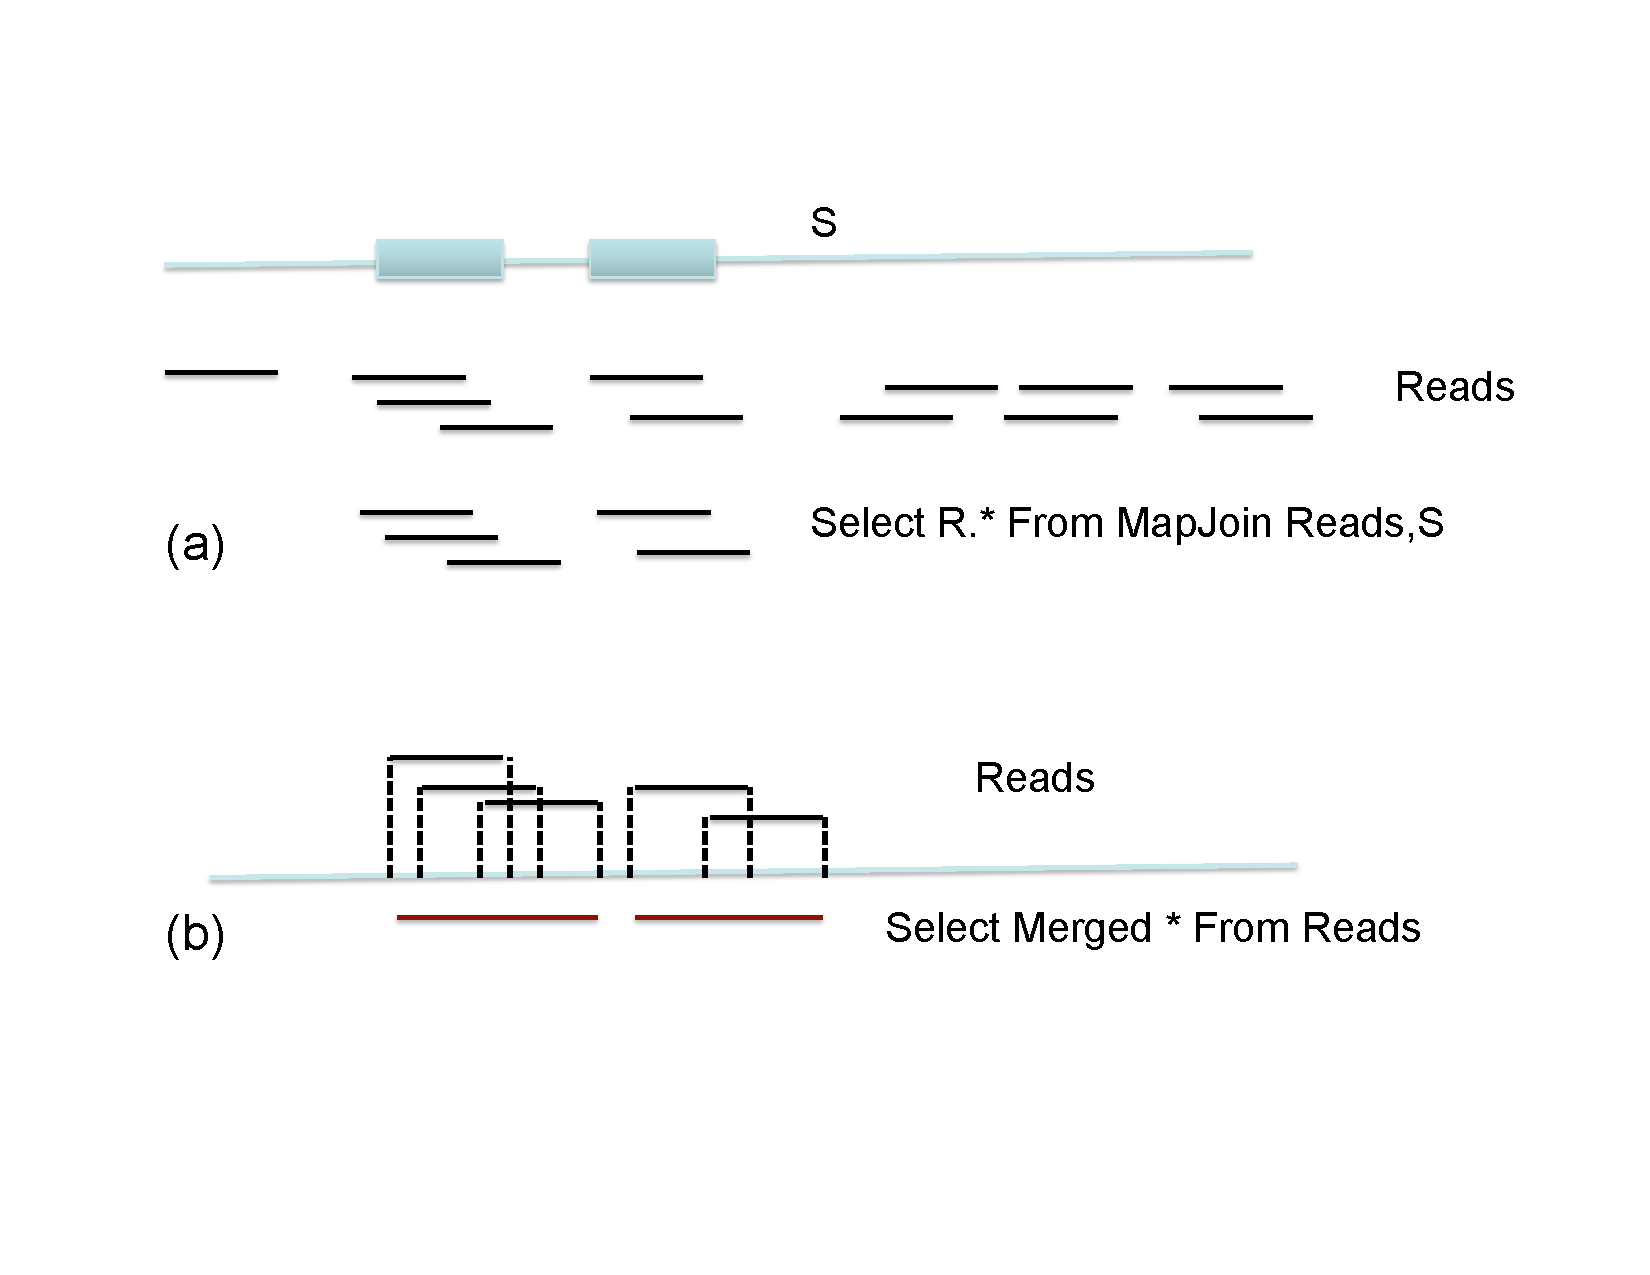
\includegraphics[trim = 20mm 50mm 10mm 10mm, clip, width=3.5in]{fig/MapJoin.pdf}
 \caption{Pictorial illustration of the MapJoin and ProjectInterval
   operations. (a) The MapJoin operation is a join based on intersection
   of intervals. In this figure, we project the reads that are in the
   MapJoin. (b) The Project Interval is expressed by the `Select Merged'
   command.}
  \label{fig:mapjoin}
\end{figure}

While geometric queries were considered for GIS databases, genomics
provides a sufficiently important domain to warrant database support
from the ground up.  We thus define a language called GQL
and show it can be used to write a number of biologically interesting
queries. GQL is based on a \emph{Genome Query Algebra-GQA}
described in the appendix.

\old{
As shown below, the key benefit of our proposed relational modeling is
to enable manipulation via algebraic operators (the standard
relational algebra operators, as well as domain-specific operators
defined shortly). This in turn creates the opportunity to leverage
proven techniques developed by the data management community for
efficiently querying large collections of data. Regardless of the fact
that some of these techniques need to be adapted or extended to our
specific domain, while others can be applied directly, the main
contribution here is to unlock the potential of large-scale data
processing in the context of a huge data scale challenge.
}

\subsection{Sample Queries} 
We have gathered many queries from practicing biologists to understand
the power of GQA. Here, we show some examples of expressive power of
the algebra. In a companion technical paper, we show that GQA's
expressive power captures the language of First Order Logic over the
relations above, as well as a signature of aggregation functions.

\begin{enumerate}

\item What is the genotype at a specific position (e.g., SNV)? 

  {\bf Query: } Let $A$ denote a relation containing the single point
  interval $\langle \mbox{chr,i,i} \rangle$. The evidence for the
  genotype at the position is provided by alignments of READS that map
  to the location, and we can either query for the mapped reads, or
  for the alignments themselves, which are often stored as a mapped
  read attribute (e.g., R.\AlignStr). Thus: 

\(\begin{array}{ll}
    \mbox{GQL:}& \mbox{\gqlSelect\  R.ID, R.\AlignStr}\\
               &\mbox{\gqlFrom\ \gqlMapjoin\ R,A}\\
  \end{array}
 \)
\item What are the diploid haplotypes (phased genotypes; see
  Section~\ref{sec:genetics}) across a set of linked loci in a
  dataset?

{\bf Query:} This is a harder query. To assemble haplotypes we need a
collection of reads each of which (perhaps along with their paired-end
reads) connect at least two polymorphic sites.  Let attribute
$R.\mbox{CloneId}$ denote the clone identifier so that the paired-end
reads $r_1,r_2$ derived from the same clone satisfy
$r_1.\mbox{CloneId}=r_2.\mbox{CloneId}$. Also, let relation $S$ denote
the collection of point intervals, one for each variant
locus.

\begin{packed_enum}
%\item Find reads and sites they map to:  
%$$RS \leftarrow R \MapRel S$$
%\item Find reads and sites {\em their partners} map to: 
%$$PS \leftarrow \Project{\attr(R)\cup\attr(S)}(\Select{\Partner(R.\ID)=P.\ID}(R \times (\rho_P(R) \MapRel S)))$$ 

\item Find a subset of READS mapping to the loci, and the count of sites the reads or their paired-ends map to (call this count $c$):\\
  \(
\begin{array}{ll}
% \mbox{GQA:}& RC \leftarrow \GrpBy{R.CloneId}{c:count()}(R\MapRel S)\\
 \mbox{GQL:}& RC = \mbox{\gqlSelect\ } R.CloneId, c=\gqlCount(*) \\
 & \mbox{ \gqlFrom\ \gqlMapjoin }R, S\\
&\hspace{0.2in} \mbox{ \gqlGroupby\ } R.CloneID\\
\end{array}
\)
\item Return \ID s of reads with count $\ge2$:\\
\(
\begin{array}{ll}
% \mbox{GQA:} &\Project{\ID}(\Select{c \geq 2}(RC))\\ 
 \mbox{GQL:} & \mbox{\gqlSelect\ } R.ID \\ 
 &\mbox{ \gqlFrom\ }R, RC\\
 &\hspace{0.2in} \mbox{ \gqlWhere\ } R.CloneID= RC.CloneID\\
 &\hspace{0.2in} \mbox{ \gqlAnd\ } (RC.c\ge 2)
\end{array}
\)
\end{packed_enum}


\item What genomic loci are affected by Copy Number Variations (CNVs)?

  {\bf Query:} If the number of donor reads mapping to a region
  exceeds some threshold $T$ then the inference might be that the
  region has been duplicated in the donor genome. Such CNVs have been
  implicated as an important variation for many disease phenotypes. To
  gather evidence, we would like all of the intervals where the number
  of mapped reads exceeds threshold $t$ (for example). Let $G.loc$
  denote a specific chromosome and location.
  \begin{packed_enum}
  \item Compute for each location, the number of reads that map to the location:\\
    \(
    \begin{array}{ll} 
%      \mbox{GQA:} & V \leftarrow \GrpBy{G.loc}{c:count()}(R \MapRel G)\\
      \mbox{GQL:} &V = \mbox{\gqlSelect\ } G.loc, c=\mbox{\gqlCount(*)}\\
        & \hspace{0.2in} \mbox{\gqlFrom\ \gqlMapjoin\ } R, G\\
      &\hspace{0.2in}\mbox{\gqlGroupby\ } G.loc
    \end{array}
    \)
  \item Return all `merged regions' where the read count exceeds threshold $t$.\\
    \(
    \begin{array}{ll}
%      \mbox{GQA:} & \ProjectInterval{G.loc} (\Select{c\ge t}(V))\\
      \mbox{GQL:} & \mbox{\gqlProjectInterval\ RS.loc}\\
      &\hspace{0.2in}\mbox{ \gqlFrom\ } V\\
      & \hspace{0.2in} \mbox{\gqlWhere\ } V.c>t
    \end{array}
    \)
  \end{packed_enum}
    

\item Identify all regions in the donor genome with large deletions.

  {\bf Query:} As discussed earlier, the evidence for deletion comes
  from a variety of sources. We use \emph{discrepant} paired-end
  mapping. Paired-end reads from clones of length $500$ (for example)
  should map $\simeq 500$bp apart on the reference genome. If instead,
  the ends happen to map \emph{discrepantly far} (e.g., $\ell$ apart
  for some $\ell>>500$, like $\ell\simeq 10000$), they support the
  case for a deletion in the donor genome. Thus, our goal is to
  identify all regions with at least $t$ discrepant paired-end reads.
  \begin{packed_enum}
  \item Use a join in which each record contains\\ the mapping locations
    of the read as well as its paired-end.\\
    \(
    \begin{array}{ll}
%      \mbox{GQA:} & H_1 \leftarrow (\Select{R.CloneID=P.CloneID}(R \times (\rho_P(R) \MapRel G)))\\
      \mbox{GQL:} &\mbox{READS already contains this join.}
    \end{array}
    \)
  \item Select records containing discrepant reads.\\
    \(
    \begin{array}{ll}
%      \mbox{GQA:} & H_2 \leftarrow \Project{R.*} \Select {|R.loc-P.loc|>10000} H_1\\
      \mbox{GQL:} &H_2= \mbox{\gqlSelect\ * \gqlFrom\ READS }\\
      & \mbox{\gqlWhere\ }abs(loc-mateloc)>10000\\
    \end{array}
    \)
  \item Select intervals containing at least $t$ discrepant reads.\\
    \(
    \begin{array}{ll}
%      \mbox{GQA:} & \ProjectInterval{G.loc}\ \Select{c>t}\ (\GrpBy{G.loc}{c:count()}\ (H_2 \MapRel G))\\
      \mbox{GQL:} & \mbox{\gqlProjectInterval\ G.loc \gqlFrom\ } H_2\\
      & \mbox{\gqlGroupby\ G.loc, c=count(*)}\\
      & \mbox{\gqlWhere\ } c>t\\
    \end{array}
    \)

  \end{packed_enum}

\end{enumerate}


\subsection{Population based queries}
The true power of querying genomes comes from the ability to query
populations. Indeed, existing tools (Samtools) allow for the ability
to extract reads from multiple individuals at specific locations
corresponding to polymorphic sites. We want to extend the full power
of genomic queries to interrogate populations. Recalling the warfarin
example, we would like to query for warfarin dosage and genetic
variation in candidate genes (genes identified through a discovery
work flow) among individuals on the warfarin regimen. Specifically, we
could be interested the following: \emph{{\bf Colloquial:} Report
  warfarin dosage and genomic intervals and reads in individuals
  s.t. the copy number of mapped reads is at least twice
  the expected coverage in the interval}.

The query for this would be similar to that of a single individual,
but repeated via a `join' with a population $P$, using\\
\(
  \begin{array}{ll}
    \mbox{GQL:} &\mbox{\gqlSelect\ * \gqlFrom\ P,\gqlMapjoin R,E }\\
    & \mbox{\gqlWhere\ P.WD = TRUE}\\
  \end{array}
  \)\\
  Using previous arguments, we can count the read depth, and report
  high CNV regions.  A similar idea applies to a \emph{personalized
    workflow}, where we would be interested in copy numbers similar to
  the specific query individual.

\old{
To gather evidence, we collect the set of reads and their copy numbers
mapping to $E$ in all individuals on a warfarin regimen. From this
set, we select the individuals and READS whose copy counts `match up'
with $p$

%Thus, we have
%\[
%W\leftarrow \GrpBy{E.loc}{c:count(R.ID)} (W) \Select{{\scriptsize \mbox{P.W}}} (P\NatJoin R\MapRel E)
%\]

%\[
%\Select{P.c\simeq p.c } W
%\] 
}

{\bf Group Inference without Accurate Individual Inference:} The
ability to query populations has an important benefit. Often,
individual genomes may have very little evidence for SNV calls at
low-coverage sequencing. However, if a large number of affected
individuals in a population (e.g., 800 out of 1000) all show the same
SNV, while controls do not, we can reliably predict an association
even with unreliable calls for individuals.  While more work is
required to demonstrate the benefits of group inference, the important
point is GQL provides query support for group inference.


\old{For individual
genomes, calling SNVs accurately is often challenging. The Inference
layer assigns quality values to individual SNV calls (e.g., SNV at Chr
10:10500 with probability 0.8), and these confidence values are used
for association with phenotypes in a segregating population.  By
contrast, population queries allow us to ask for evidence about
arbitrary subsets of large groups of users based on various
characteristics of these users and doing statistical inference
directly on these large groups. They allow us to bypass the
determination of individual SNVs. 
}


\section{A prototype implementation}
We have developed a prototype implementation, \emph{genomequery} of a
subset of GQL (Figure~\ref{fig:genomequery}). The uploaded genome (in
BAM format) can be queried using a simple text interface that allows
the user to write a GQL query. The query is compiled and executed, and
the output returned as a (smaller) BAM file that can be visualized
using jbrowse, or downloaded to the client for further analysis.

\begin{figure}[ht]
  \centering
  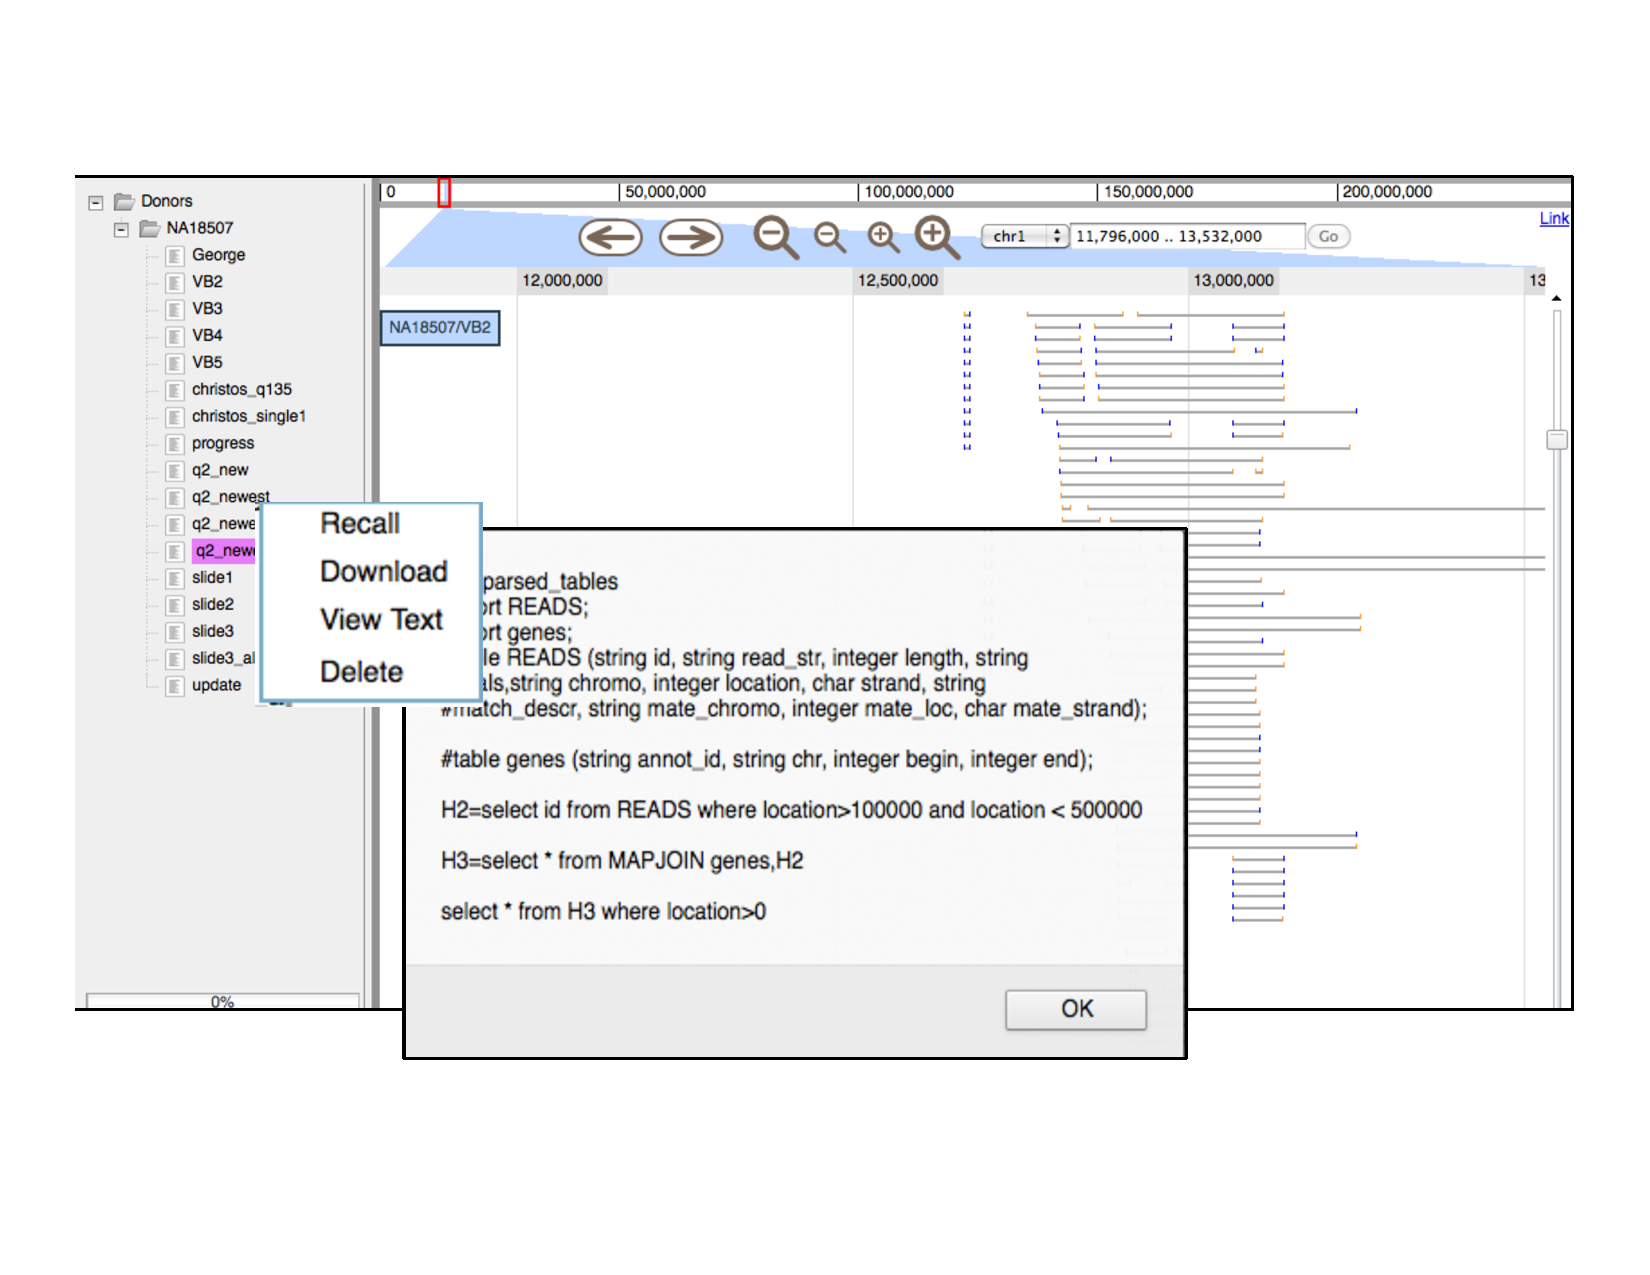
\includegraphics[trim = 10mm 35mm 10mm 25mm, clip,width=3.5in]{fig/genomequery.pdf}
  \caption{A prototype implementation of GQL, with visualization using
    the open source tool jbrowse. Discordant paired-end reads
    supporting deletions can be seen.}
  \label{fig:genomequery}
\end{figure}
The implementation of \emph{genomequery} has a customized parser that
converts GQL to an intermediate representation resembling GQA. Thus,
there are customized procedures for each of the algebraic operations,
with some concessions for efficiency (mainly w.r.t
memory). Specifically, we use interval trees to implement $\MapRel$,
and customized indices (including Strength Vectors; see below) for
efficient querying. Details on the implementation will be provided
elsewhere. 

\section{The way forward: challenges for computer scientists}
\label{sec:futuredirections}
So far we have made the case for a set of genomic layers,
including an Evidence Layer where evidence is retrieved
using a Genome Query Language. Successful implementation of this
vision will depend upon some new ideas from computer science: 
specific areas are marked in the subsection titles

\subsection{Query Power -- Database Theory}
Is GQL sufficiently
powerful to address all Evidence Layer queries needed in practice? 
The goal is to have the
Evidence Layer handle as much of the data-intensive computation as possible
while preserving performance; without the performance goal, any
query can be trivially satisfied by passing the entire genome to the
inference layer.  It helps to note that GQL's expressive power
coincides with that of first order logic over the schema of the three
relations $R,G,P$, a signature of aggregation functions, and a
group-by operator.  However, user feedback may require
extensions. In implementing extensions, care must be taken to balance
expressive power with efficient evaluation. 

\subsection{Query Speed  --- Database Systems}
We have designed a corresponding algebra GQA
as an internal representation for
optimization and evaluating query plans.  
As an example, assume that queries on populations will automatically
be decomposed into queries on individuals. Consider queries of the
general form \gqlSelect $\:a\:$ \gqlFrom $\:$ \gqlMapjoin $\:R,G\:$
\gqlWhere $\:b$. The two steps are
%\begin{enumerate}
\begin{packed_enum}
\item Select for relations that satisfy constraints $b$.
\item Project (while removing duplicates) on to attributes $a$.
\end{packed_enum}
%\end{enumerate}
We use a location based index {\sc LtoR}, where {\sc LtoR}$(\ell)$ is
a pointer to first read that maps to the point-interval $l$. For
each individual, we keep a compressed index of the mapped reads in
memory. The index can be used for Select operations based on specific
locations (e.g, reads that map to specific genes).

However many queries involve scanning the entire genome for maximal
intervals. For example, find all maximal regions where there is a
disproportionate increase in the number of mapped reads (High copy
number).   For efficient implementation of these queries, we construct special
indices that allow filtering for READS according to a user-defined
constraint. Define a {\em strength vector} $S_{\theta}$ for a
constraint $\theta$ as a vector of length $G$ (the entire genome).
For any location $\ell \in G$, $S_{\theta}[\ell]$ gives the
strength of the evidence at that location, and can be precomputed for
common constraints $\theta$.  To reduce memory, we also choose a
minimum strength cut-off, and maintain $C_{\theta,t}$ as a sorted
sequence of intervals $i_1, i_2, \ldots$ such that each $i_j$ is a
maximal interval satisfying $S_{\theta}[\ell] \geq t$ for all $\ell\in
i_j$.  The compressed vectors reduce memory and computation
requirements and can be recomputed on demand.

\old{
If the compressed strength vector is $100\times$ smaller than the
strength vector, it will be correspondingly faster to read it off
disk.  For large populations, where the compressed strength vectors
must be loaded off the disk iteratively, this offers a great speed
advantage. The trick is to choose thresholds appropriately so that the
inference layer can get a superset of what it needs, but that is still
smaller than the set of all READS. 

Consider the query from before
\[
   \Project{g}\:\: \Select{{\scriptsize \mbox{p.d {\sc and} HighCNV}(R,g)}} (P\NatJoin R\MapRel G)
\]
We use the natural join $P\NatJoin R$ select all records corresponding
to individuals satisfying ``p.d'' and project out the corresponding
pointers to their compressed strength vectors. We now traverse each
compressed strength vector, incrementing the count for each location
spanned by subinterval $i$ of the compressed strength vector for
patient $j$.  We keep track in an output queue of all locations whose
counts are over some threshold $r$.  It should be clear that this can
be generalized to more sophisticated queries (e.g., locations in which
$X\%$ of patients have high copy number and$Y\%$ of non-patients have
low copy number). 
}

\subsection{EMRs -- Information Retrieval}
The phenotypes associated with each sequenced individual are already
in patient medical records. Initial results from the eMERGE network
indicate that, for a limited set of diseases, it is possible to
utilize the EMR for phenotype characterization in genome wide
association studies (GWAS) within a reasonable margin of
error\cite{Kho2011,Pathak2011}. It is anticipated that most
healthcare institutions will be utilizing EMRs by 2014, given
incentives provided by the HITECH act\cite{Stark2010}. Increasing
adherence to interoperability standards\cite{Dolin2011} and advances
in biomedical natural language processing\cite{Nadkarni2011}, make
efficient querying possible. However, there is currently no
integration of genotype and phenotype data. GQL should be useful both
for interrogating a single genome or interrogating several genomes
across groups of individuals, but will need to integrate with existing
EMR systems so that phenotype data could be queried together with
genomes.

\subsection{Privacy -- Computer Security}
The genome is the ultimate unique identifier. All privacy is lost once
we have access to the genome of an indvidual, but the current
regulation, the Health Information Portability and Accountability Act
(HIPAA) is silent about this
identifier\cite{Annas2003,Benitez2010,Malin2011}. Although the Genetic
Information Nondiscriminating Act (GINA) addresses accountability for
use of genetic information\cite{Hudson2008}, privacy laws will need to
change to ensure that sensitive information is available only to the
appropriate person. Checking that a given study satisfies a specific
privacy definition requires formal reasoning about the data
manipulations that generated the disclosed data, which is impossible
without a declarative specification of such manipulations. This is
exactly what GQL queries offer. Current efforts involve the
investigation of differential privacy\cite{Chaudhuri2011}, as well as
multiple types of de-identification
procedures\cite{OhnoMachado2004,OhnoMachado2011}. 

\old{While this is not
within the scope of this article, GQL at least enables a design
process to start. Typically, such a design process for privacy
measures tries to maximize the class of allowable study outputs.
}

\subsection{Provenance -- Software Engineering}
GQL is an ideal vehicle for recording provenance of study conclusions.
Current scripts often consist of code that is often too ad-hoc for
human readability, and span various programming languages, too
low-level for automatic analysis. In contrast,
publishing the set of declarative GQL queries along with their results
would significantly enhance the clarity and reproducability of a study's claims.

\old{
The
declarative nature of such queries renders them orders of magnitude
more readable by humans and programs than the scripts used currently
to code the data manipulations. Such s

Storing study provenance as queries also
paves the way for tools that react automatically when the input data to
the study changes (an all too common event).  This happens when the
input data producer (possibly a set of autonomous third-party labs),
adds new data entries, or retracts or corrects old ones.  By analyzing
the query expressions, changes to the study's input data can be
automatically propagated to the output in an incremental fashion,
without re-running the entire expensive query from scratch.  The
relational analogy to this scenario is known in the database literature
as 'incremental view updating', and is being used successfully in data
warehousing applications.
}
 
Provenance queries also enable scientists to reuse the data of previously
published computing-intensive studies. Instead of running her
expensive queries directly on the original input databases, the
investigator would launch an automatic search for previously published
studies whose provenance queries correspond to (parts of) the
computation needed by her own queries.  The results of the provenance
queries can be directly imported and used as partial results of the
new study's queries, skipping re-computation.  This scenario
corresponds in relational database practice to that of 'rewriting
queries using views'.

\subsection{Discovery at Scale --- Probabilistic Inference}
Learning the correlation between diseases and variations
can be tackled differently if there are a large number of genomes.  It may
be less critical to accurately evaluate individual variations for such a discovery problem,
because erroneous variations are unlikely to occur over a large group of randomly
chosen individuals.   More generally, what other inference techniques are there that
leverage the presence of data at scale.   As an example, Google leverages the large
data it has to find common misspellings.   Note that accurately screening individual
variations is still needed for personalized medicine. 

\subsection{Crowd-sourcing --- Data Mining}
Patterson suggests the use of crowd-sourcing
techniques to solve hard challenges like
cancer\cite{Patterson2011}. To enable this, the query system must have
mechanisms to allow a group to work coherently on a problem.
For example, imagine that talented high school science
students look for genetic associations using genomes from cases and
controls for specific diseases. A mechanism that could be useful is
the selection of a \emph{random} subset of cases and controls, which
are nevertheless genetically matched (arising from a single, mixing
population). Then, instead of selecting from all (tens of thousands of)
individuals, one could query for a random subset of $100$ individuals
using a fraction of network bandwidth, while still providing similar
statistical power for detecting associations.


\subsection{Reducing Costs -- Computer Systems}

Personalized medicine must be commoditized to be
successful; this requires computer systems research.
For example, since most genomes are read only, could
solid-state disks (SSDs) be leveraged?  Second, efficient decomposition 
between the cloud and the
workstation is key to reducing data traffic in and out of the
cloud.  Third, while genomics has been
dominated historically by expensive parallel computers, it makes
economic sense to adapt genomic software to harness
the parallelism present in cheap multicore CPUs.


\section{Conclusion}
\label{sec:conclusion}

Genomics is moving from an era of scarcity (a few genomes with
imperfect coverage) to abundance (universal sequencing with high
coverage and cheap resequencing when needed).  This shift requires
rethinking genomic processing from ad hoc tools that
support a few scientists to commodity software that can support a
world of medicine.  The history of computer systems teaches us that as
systems move from scarcity to abundance, modularity is paramount; ad
hoc software must replaced by a set of layers with well defined
interfaces.   That these trends have been
recognized by industry can be seen by the shift from machine specific
formats such as Illumina to standards such as BAM, and from vendor
specific variant formats to VCF.  The 1000 genomes project has gained
momentum and a large number of sequences are already accessible.
However, much of the progress today has been to define data formats
without powerful interface functionality; to use an Internet analogy
this is as if TCP packet formats were defined without the socket
interface.

Our paper proposes going beyond the layering implicit in current
industry standards to enable
personalized medicine and discovery.  We advocate the
separation of evidence from inference, and the separation of
individual variation from variation across groups
(Figure~\ref{fig:abstraction}a)).  More concretely, we propose a
specific interface between the EL and the IL via a Genome Query
Language (GQL).  While GQL is based on a relational model using a
virtual interval relation, we have found that effort is required
beyond standard relational optimization to allow GQL to scale to large
genomes and large populations.

We described several benefits to separating evidence from inference.
A genome repository accessible by GQL offers the ability to reuse
genomic data across studies, the ability to logically assemble
case-control cohorts, and the ability to rapidly change queries
without ad-hoc programming.  GQL also offers the
ability to reduce the quality of inference on an individual basis when
doing group inference on large populations.
We described some simple ideas to scale GQL to populations using
compressed strength indices and by doing EL processing in the cloud.

We emphasize that GQL and the EL are only our initial attempt at capturing abstractions
for genomics.  We hope our paper starts a larger conversation between computer scientists
and biologists to tease out the right interfaces and layers for medical applications
of genomics.  Beyond abstractions, much work remains to be done to complete the vision
including better large scale inference, system optimizations to
increase efficiency, information retrieval to make medical records
computer readable, and security mechanisms.  While the work is vast,
so is the opportunity.  It is not often that computer scientists get a chance to
work on a large system such as the Internet or UNIX that can change
the world.

\section{Acknowledgment}
The authors acknowledge support from the NIH sponsored iDASH project
(Grant U54 HL108460), NIH 5R01-HG004962, and a CSRO scholarship to
CK.  We thank Rajesh Gupta, Vish Krishnan,
Ramesh Rao, and Larry Smarr for useful discussions and support.

\bibliographystyle{abbrv}
\bibliography{query.bib}

\newpage
\section{Appendix}

Our database has some key relations. The first is \emph{R (Reads)}
that describe the set of read fragments output by the sequencer, and
all of their properties.  For example, for paired-end sequencing, $R$
could contain identifiers for each read $r$, and its paired-end. A
second relation encodes a set of intervals on the genome, where each
is specified by the triple ``$\langle\mbox{chromosome, start-position,
  end-position} \rangle$''. A specific, and important, case of the
interval relation is the relation $G$ (the genome) where each entry is
a point interval corresponding to a specific location ({\em locus })
on the genome. As $G$ is large ($3\cdot 10^9$ loci), we do not
materialize $G$ explicitly, using it instead as a virtual (conceptual)
relation to facilitate the relational expression of queries. A final
relation $P$ describes the set of all individuals in a population, and
will be discussed in a subsequent section.



{\bf Standard relational algebra operators and language
  constructs}
Standard algebraic operators we use in the examples below include: 
\begin{packed_itemize}
\item The projection operator $\Project{}$ where $\Project{X}(E)$
  returns, from the relation $E$ evaluates to, the restriction of the
  tuples to the attributes named in $X$. In GQL, we express this
  operation using
  \[
  \mbox{\gqlSelect\ } \mbox{X}  \mbox{ \gqlFrom\ }  E
  \]
\item The selection operator $\Select{}$, where $\Select{\theta}(E)$
  selects the subset of precisely those tuples in the result of
  expression $E$ that satisfy filter predicate
  $\theta$. Correspondingly, in GQL:
  \[
  \mbox{\gqlSelect\ * \gqlFrom\  E \gqlWhere\ } \theta
  \]
\item The Cartesian product operator $\times$, where $E\times F$
  refers to all tuples of the form $(e,f)$ where $e\in E, f\in F$. In
  GQL:
  \[
    \mbox{\gqlSelect\ * \gqlFrom\  E,F}
  \]

\item The renaming operator $\rho_N(E)$, which sets to $N$ the name of
  the relation returned by $E$.
\item The group-by operator $\GrpBy{}{}$, where in
  $\GrpBy{G_1,G_2,\ldots,G_k}{N_1:F_1(A_1),\ldots,N_l:F_l(A_l)}(E)$,
  $E$ is an algebraic expression that evaluates to a relation,
  $G_1,\ldots,G_k$ are group-by attributes, each $F_i$ is an aggregate
  function and each $N_i,A_i$ are attribute names.  The meaning of the
  group-by operator is the standard one: all tuples in the result of
  $E$ are partitioned into groups, such that two tuples are in the
  same group if and only if they agree on the values of all group-by
  attributes.  Thus, the groups can be identified by the value of the
  group-by attributes.  For each group $(g_1,\ldots,g_k)$, the result
  contains a tuple of attributes $G_1,\ldots,G_k,N_1,\ldots,N_l$ and
  values $(g_1,\ldots,g_k,n_1,\ldots,n_l)$, respectively. Here, each
  $n_i$ is computed by applying function $F_i$ to the collection of
  attribute $A_i$'s values found in the group. In GQL:
\[
  \begin{array}{l}
    \mbox{\gqlSelect\ } G_1,\ldots,G_k,N_1=F_1(A_1),\ldots,N_l=F_l(A_l) \mbox{ \gqlFrom\ }  E\\ 
    \mbox{\gqlGroupby\ } G_1,\ldots G_k
  \end{array}
\]



By default, this
  collection is viewed as a multiset, i.e. duplicate values are not
  removed.  To apply $F_i$ after eliminating duplicates, we use the
  syntax $N_i:F_i(\mbox{distinct\ } A_i)$.  The syntax of the count
  aggregation is an exception, in that no $A_i$ attribute need be
  specified.
\end{packed_itemize}


{\bf The Map join and the Project Interval operator:}
As reads are sequenced, they are also mapped to the reference genome
using various mapping algorithms. Some mapping algorithms map each
read to a unique location, or not at all; others may choose to
identify all intervals where the underlying genomic string is similar
(in terms of edit distance) to the read. For now, assume that each
read is mapped to its best location by a mapping algorithm $M$, and
the relation $R$ includes the interval of the best map.
\old{ (i.e. $\ID \subseteq \attr(R)$, where $\attr(R)$ denotes the set
  of $R$'s attributes). Note that under this assumption, the \ID\
  attributes uniquely identify each read (tuple in $R$).}


For an arbitrary relation of genomic intervals, $A$, define a
\emph{map-join} operation $R\MapRel A$ by a pair of tuples $(r,g)\in
R\times A$ such that (r.chr, r.start, r.end) and (a.chr, a.start,
a.end) `intersect'. Recall that we defined the relation $G$ as the set
of all genomic loci. Therefore, $R\MapRel G$, denotes the set of all
tuples $r,g$ where $g$ denotes a genomic coordinate that $r$ maps to.
In many practical instances, the relation is quite large. If 33\% of
the genome was mapped on the average by 10 reads, $R\MapRel G$ would
contain $\simeq \frac{1}{3} 3\cdot 10^9\cdot 10= 10^{10}$ tuples. In
GQL:
\[
    \mbox{\gqlSelect\ } * \mbox{ \gqlFrom\ \gqlMapjoin\ }  R,G\\ 
\]


To reduce output size, we define a special \emph{Project-interval}
operator $\ProjectInterval{}$. $\ProjectInterval{A.ID} (R\MapRel A)$
outputs all genomic intervals after `fusing' adjacent and overlapping
intervals. Thus,
\[
\ProjectInterval{G.ID} (R\MapRel G)
\] 
would result in the set of all disjoint genomic intervals with some
read mapping to them. Correspondingly, in GQL:
\[
    \mbox{\gqlProjectInterval\ G.ID} \mbox{ \gqlFrom\ \gqlMapjoin\ }  R,G\\ 
\]

\end{document}
